\documentclass[12pt,a4paper]{article}
\usepackage[T1]{fontenc}
\usepackage[utf8]{inputenc}
\usepackage{lmodern}
\usepackage{amsmath,amssymb,amsthm,mathtools}
\usepackage{geometry}
\geometry{margin=1in}
\usepackage{microtype}
\usepackage{hyperref}
\usepackage{xcolor}
\usepackage{enumitem}
\usepackage{fancyhdr}
\usepackage{bookmark}
\usepackage{array}

\usepackage{float}

\usepackage{centernot}

\DeclareMathOperator{\rank}{rank}

\DeclareMathOperator{\Deck}{Deck}

\usepackage{tikz-cd}

\usepackage{tocloft}
\setlength{\cftsubsecnumwidth}{3.2em}

\newtheorem{prop}{Proposition}[section]

\newcommand{\Q}{\mathbb{Q}}
\newcommand{\RP}{\mathbb{R}\mathrm{P}}

\newcommand{\Z}{\mathbb{Z}}

\newcommand{\Chi}{\chi}
\newcommand{\del}{\partial}

\newtheorem{definition}{Definition}[section]

\newtheorem{example}[definition]{Example}

\hypersetup{
	colorlinks=true,
	linkcolor=blue!50!black,
	urlcolor=blue!50!black,
	citecolor=blue!50!black,
	pdftitle={Theory of Algebraic Topology 11},
	pdfauthor={},
	pdfsubject={Solved problems and theory notes in commutative algebra},
	pdfcreator={OpenAI}
}

\setlist[itemize]{topsep=4pt,itemsep=2pt,parsep=0pt,partopsep=0pt}
\setlength{\parskip}{0.55em}
\setlength{\parindent}{0pt}

\setcounter{secnumdepth}{2}


\setcounter{tocdepth}{2}

\pagestyle{fancy}


\usepackage{tikz}
\usetikzlibrary{positioning}

\fancyhf{}
\lhead{Theory of Algebraic Topology 11}
\rhead{\thepage}
\renewcommand{\headrulewidth}{0.4pt}

\newtheoremstyle{notespace}{6pt}{6pt}{\normalfont}{} {\bfseries}{.}{0.5em}{}
\theoremstyle{notespace}

\newtheorem{remark}{Remark}[section]

\DeclareMathOperator{\Spec}{Spec}
\DeclareMathOperator{\Ass}{Ass}
\DeclareMathOperator{\Ann}{Ann}
\DeclareMathOperator{\Supp}{Supp}
\DeclareMathOperator{\Hom}{Hom}
\DeclareMathOperator{\Min}{Min}
\DeclareMathOperator{\Ker}{Ker}
\DeclareMathOperator{\Frac}{Frac}

\DeclareMathOperator{\depth}{depth}
\DeclareMathOperator{\Tor}{Tor}
\DeclareMathOperator{\Ext}{Ext}

\DeclareMathOperator{\coker}{coker}
\DeclareMathOperator{\im}{im}

\newcommand{\longdash}{\mathrel{\text{---}}}

\title{\vspace{-1.5em}\bfseries Theory of Algebraic Topology 11}
\author{}
\date{\today}

\begin{document}
	\maketitle
	\thispagestyle{plain}
		\begin{center}
		\begin{minipage}{0.92\textwidth}
			Lecture notes with worked examples in algebraic topology
		\end{minipage}
	\end{center}
		\pdfbookmark[1]{Contents}{contents}\tableofcontents
	\clearpage

\section{Problem 1 Homotopic attaching maps give the same homotopy type}

\paragraph{Statement.}
If \(f_0,f_1:S^{n-1}\to X\) and \(f_0\simeq f_1\), show that
\[
X\cup_{f_0} D^n \simeq X\cup_{f_1} D^n .
\]

\paragraph{Solution.}
This is a standard fact about attaching cells: attaching an \(n\)-cell along two homotopic maps produces homotopy equivalent spaces.

Write
\[
Y_i:=X\cup_{f_i}D^n \qquad (i=0,1).
\]
Each \(Y_i\) is the pushout of the diagram
\[
\begin{tikzcd}
	S^{n-1} \arrow[r,"f_i"] \arrow[d,hook] & X \arrow[d] \\
	D^n \arrow[r] & Y_i .
\end{tikzcd}
\]

Now let
\[
H:S^{n-1}\times I \to X
\]
be a homotopy from \(f_0\) to \(f_1\), so
\[
H(-,0)=f_0,\qquad H(-,1)=f_1.
\]

The key point is that the inclusion
\[
S^{n-1}\hookrightarrow D^n
\]
is a \emph{cofibration}. For cofibrations, ordinary pushouts agree with homotopy pushouts. Therefore the homotopy type of the adjunction space depends only on the homotopy class of the attaching map.

Equivalently, the two pushout diagrams
\[
\begin{tikzcd}
	S^{n-1} \arrow[r,"f_0"] \arrow[d,hook] & X \arrow[d] \\
	D^n \arrow[r] & X\cup_{f_0}D^n
\end{tikzcd}
\qquad\text{and}\qquad
\begin{tikzcd}
	S^{n-1} \arrow[r,"f_1"] \arrow[d,hook] & X \arrow[d] \\
	D^n \arrow[r] & X\cup_{f_1}D^n
\end{tikzcd}
\]
have the same homotopy type because \(f_0\) and \(f_1\) are homotopic.

Hence
\[
X\cup_{f_0}D^n \simeq X\cup_{f_1}D^n.
\]

\paragraph{Remark.}
This is one of the basic principles behind CW-complexes: the homotopy type of a CW-complex depends only on the homotopy classes of its attaching maps, not on the precise representatives.

\bigskip

\section{Problem 2 A CW structure on \(S^n\) with two cells in each dimension}

\paragraph{Statement.}
Consider the cell structure on \(S^n\) having two cells of dimension \(k\) for each \(0\le k\le n\), coming from the northern and southern hemispheres of
\[
S^k\subset S^n .
\]
Write out its cellular chain complex and verify that it gives the correct homology of \(S^n\).

\paragraph{Description of the CW structure.}
For each \(k=0,1,\dots,n\), let
\[
e^k_+,\ e^k_-
\]
denote the open northern and southern hemispheres of \(S^k\subset S^n\). Then
\[
S^k = e^k_+ \cup e^k_- \cup S^{k-1},
\]
so the \(k\)-skeleton is exactly
\[
X^k=S^k.
\]
Thus this really is a CW structure on \(S^n\), with two \(k\)-cells for every \(0\le k\le n\).

\paragraph{Cellular chain groups.}
Since \(X^k=S^k\) and \(X^{k-1}=S^{k-1}\), we have
\[
C_k^{\mathrm{cell}}(S^n)=H_k(X^k,X^{k-1})=H_k(S^k,S^{k-1}).
\]
Now collapsing the equator \(S^{k-1}\subset S^k\) gives the wedge of two \(k\)-spheres:
\[
S^k/S^{k-1}\cong S^k\vee S^k.
\]
Therefore
\[
C_k^{\mathrm{cell}}(S^n)\cong \widetilde H_k(S^k\vee S^k)\cong \mathbb Z\oplus \mathbb Z,
\qquad 0\le k\le n.
\]
We use the basis
\[
C_k=\mathbb Z\langle e^k_+,e^k_-\rangle .
\]

\paragraph{Boundary maps.}
With a suitable choice of orientations on the cells, the cellular boundary maps are
\[
\partial_k(e^k_+) = e^{k-1}_+ - e^{k-1}_-,\qquad
\partial_k(e^k_-) = e^{k-1}_+ - e^{k-1}_-
\]
for every \(k\ge 1\).

So, with respect to the ordered bases \((e^k_+,e^k_-)\) and \((e^{k-1}_+,e^{k-1}_-)\), the matrix of \(\partial_k\) is
\[
\partial_k=
\begin{pmatrix}
	1 & 1\\
	-1 & -1
\end{pmatrix}
\qquad (k\ge 1).
\]

Thus the cellular chain complex is
\[
0\longrightarrow \mathbb Z^2
\xrightarrow{\ \partial_n\ }
\mathbb Z^2
\xrightarrow{\ \partial_{n-1}\ }
\cdots
\xrightarrow{\ \partial_2\ }
\mathbb Z^2
\xrightarrow{\ \partial_1\ }
\mathbb Z^2
\longrightarrow 0,
\]
with every differential given by the same matrix
\[
\begin{pmatrix}
	1 & 1\\
	-1 & -1
\end{pmatrix}.
\]

\paragraph{Check that \(\partial_{k-1}\partial_k=0\).}
Indeed,
\[
\begin{pmatrix}
	1 & 1\\
	-1 & -1
\end{pmatrix}
\begin{pmatrix}
	1 & 1\\
	-1 & -1
\end{pmatrix}
=
\begin{pmatrix}
	0 & 0\\
	0 & 0
\end{pmatrix},
\]
so this is a genuine chain complex.

\paragraph{Compute the homology.}
For each \(k\ge 1\),
\[
\ker \partial_k
=
\{(a,b)\in \mathbb Z^2 : a+b=0\}
=
\mathbb Z\langle e^k_+ - e^k_- \rangle.
\]
Also,
\[
\operatorname{im}\partial_{k+1}
=
\mathbb Z\langle e^k_+ - e^k_- \rangle.
\]
Hence for every middle dimension \(1\le k\le n-1\),
\[
H_k(S^n)=\ker \partial_k/\operatorname{im}\partial_{k+1}=0.
\]

At the top dimension,
\[
H_n(S^n)=\ker \partial_n
=
\mathbb Z\langle e^n_+ - e^n_- \rangle
\cong \mathbb Z,
\]
since \(C_{n+1}=0\).

At dimension \(0\),
\[
H_0(S^n)=C_0/\operatorname{im}\partial_1.
\]
But
\[
\operatorname{im}\partial_1
=
\mathbb Z\langle e^0_+ - e^0_- \rangle,
\]
so in \(H_0\) the two \(0\)-cells become identified, and therefore
\[
H_0(S^n)\cong \mathbb Z.
\]

So the cellular homology is
\[
H_k(S^n)\cong
\begin{cases}
	\mathbb Z, & k=0,n,\\[4pt]
	0, & 0<k<n,
\end{cases}
\]
which is exactly the correct homology of the sphere \(S^n\).

\paragraph{Final remark.}
Different choices of orientations may change some signs in the matrices, but all such chain complexes are isomorphic and give the same homology.


\section{Theory for Problems 1 and 2}

\subsection{Attaching a cell along homotopic maps}

\subsubsection{Attaching an \(n\)-cell}

A fundamental construction in algebraic topology is to start with a space \(X\), take a closed disk \(D^n\), and glue its boundary sphere
\[
S^{n-1}=\partial D^n
\]
to \(X\) by a continuous map
\[
f:S^{n-1}\to X.
\]
The resulting space is denoted by
\[
X\cup_f D^n
\]
and is called an \emph{adjunction space} or the space obtained from \(X\) by \emph{attaching an \(n\)-cell}.

Formally,
\[
X\cup_f D^n=(X\sqcup D^n)/\sim,
\]
where for each \(x\in S^{n-1}\subset D^n\) we identify
\[
x\sim f(x)\in X.
\]
Thus the topology of the new space is determined by the way the boundary of the disk is attached to \(X\).

\subsubsection{Why the attaching map matters}

The attaching map can change the topology of the resulting space in an essential way. For example, if \(X=\{*\}\) is a point, then attaching \(D^n\) to that point collapses the whole boundary sphere, so
\[
\{*\}\cup_f D^n \cong D^n/S^{n-1}\cong S^n.
\]
On the other hand, if \(X=S^1\) and we attach a \(2\)-cell by a map of degree \(m\),
the resulting space has first homology group \(\mathbb Z/m\mathbb Z\). Hence different attaching maps may produce non-homeomorphic and even non-homotopy-equivalent spaces.

\subsubsection{Homotopy class of the attaching map}

Although the exact attaching map matters topologically, from the point of view of homotopy theory only its homotopy class matters. More precisely, if
\[
f_0,f_1:S^{n-1}\to X
\]
are homotopic, then
\[
X\cup_{f_0}D^n \simeq X\cup_{f_1}D^n.
\]
This is the basic content behind Problem 1.

So when one attaches a cell to a space, the resulting homotopy type depends only on the class
\[
[f]\in [S^{n-1},X].
\]
This fact is one of the central principles in CW-complex theory.

\subsubsection{The role of cofibrations}

The conceptual reason behind the homotopy invariance above is that the inclusion
\[
S^{n-1}\hookrightarrow D^n
\]
is a \emph{cofibration}. Cofibrations have the homotopy extension property, which informally means that homotopies defined on the subspace extend well to the larger space. Because of this, pushouts formed along cofibrations behave well with respect to homotopies.

A general principle is:

\begin{quote}
	Pushouts along cofibrations are homotopy-invariant.
\end{quote}

Problem 1 is a very important special case of this principle. Since \(S^{n-1}\hookrightarrow D^n\) is a cofibration, replacing the attaching map by a homotopic one does not change the homotopy type of the resulting adjunction space.

\subsubsection{Geometric intuition}

Suppose
\[
H:S^{n-1}\times I\to X
\]
is a homotopy from \(f_0\) to \(f_1\). Then one may imagine the boundary of the disk gradually sliding through \(X\), changing the attachment from \(f_0\) to \(f_1\). The interior of the disk remains an \(n\)-cell; only the way its boundary is glued changes continuously.

Since this change happens through a homotopy, the resulting spaces are homotopy equivalent. Thus changing the attaching map continuously does not change the essential homotopy type of the space.

\subsubsection{Importance for CW-complexes}

CW-complexes are built inductively:
\begin{itemize}
	\item begin with \(0\)-cells,
	\item attach \(1\)-cells,
	\item then attach \(2\)-cells,
	\item and continue in higher dimensions.
\end{itemize}

At each stage one attaches cells by maps
\[
S^{n-1}\to X^{n-1},
\]
where \(X^{n-1}\) is the previous skeleton. The fact proved in Problem 1 shows that the homotopy type of the resulting CW-complex depends only on the homotopy classes of these attaching maps. This is one of the reasons CW-complexes are such a powerful framework in algebraic topology.

\subsection{A CW structure on \(S^n\) with two cells in each dimension}

\subsubsection{CW structures are not unique}

A topological space can admit many different CW decompositions. In particular, the sphere \(S^n\) has a very small CW structure consisting of
\begin{itemize}
	\item one \(0\)-cell,
	\item one \(n\)-cell,
	\item no cells in intermediate dimensions.
\end{itemize}

However, \(S^n\) can also be given richer CW structures with many more cells. Problem 2 considers such a decomposition: for each \(k\) with \(0\le k\le n\), there are two \(k\)-cells, coming from the northern and southern hemispheres of \(S^k\subset S^n\).

This example is important because it shows that CW structures are not unique, but cellular homology still computes the same homology of the underlying space.

\subsubsection{The hemisphere decomposition of \(S^k\)}

For each \(k\ge 1\), the sphere \(S^k\) may be written as
\[
S^k=D^k_+\cup D^k_-,
\qquad
D^k_+\cap D^k_-=S^{k-1},
\]
where \(D^k_+\) and \(D^k_-\) are the northern and southern closed hemispheres.

Their interiors are open \(k\)-cells, which we denote by
\[
e_+^k,\qquad e_-^k.
\]
Thus \(S^k\) is obtained from \(S^{k-1}\) by attaching two \(k\)-cells. Repeating this construction through the chain
\[
S^0\subset S^1\subset \cdots \subset S^n
\]
gives a CW decomposition of \(S^n\) in which
\[
X^k=S^k
\]
is the \(k\)-skeleton and there are exactly two cells in each dimension \(k\).

\subsubsection{Cellular chain groups}

If \(X\) is a CW-complex, its cellular chain groups are defined by
\[
C_k^{\mathrm{cell}}(X)=H_k(X^k,X^{k-1}).
\]
If there are \(r_k\) cells of dimension \(k\), then
\[
C_k^{\mathrm{cell}}(X)\cong \mathbb Z^{r_k}.
\]

In the CW structure of Problem 2 there are two cells in each dimension, so
\[
C_k^{\mathrm{cell}}(S^n)\cong \mathbb Z^2
\qquad (0\le k\le n).
\]
A natural basis is given by the two cells
\[
e_+^k,\qquad e_-^k.
\]

Thus the cellular chain complex has the form
\[
0\to \mathbb Z^2 \xrightarrow{\partial_n} \mathbb Z^2 \xrightarrow{\partial_{n-1}} \cdots
\xrightarrow{\partial_2}\mathbb Z^2\xrightarrow{\partial_1}\mathbb Z^2\to 0.
\]

\subsubsection{Why the relative homology is \(\mathbb Z^2\)}

Since in this CW structure
\[
X^k=S^k,\qquad X^{k-1}=S^{k-1},
\]
we have
\[
C_k=H_k(S^k,S^{k-1}).
\]
Now collapse \(S^{k-1}\subset S^k\) to a point. The two hemispheres of \(S^k\) then become two copies of \(S^k\) joined at one point, so
\[
S^k/S^{k-1}\cong S^k\vee S^k.
\]
Therefore
\[
H_k(S^k,S^{k-1})
\cong \widetilde H_k(S^k/S^{k-1})
\cong \widetilde H_k(S^k\vee S^k)
\cong \mathbb Z\oplus \mathbb Z.
\]
This gives a geometric explanation for the fact that there are two generators in each cellular chain group.

\subsubsection{The cellular boundary maps}

The cellular boundary map
\[
\partial_k:C_k\to C_{k-1}
\]
records how the boundary of each \(k\)-cell wraps around the \((k-1)\)-skeleton. In this hemisphere decomposition, each \(k\)-cell has equatorial boundary \(S^{k-1}\), and the cellular boundary of each hemisphere is the difference of the two \((k-1)\)-cells.

With a suitable choice of orientations, one gets
\[
\partial_k(e_+^k)=e_+^{k-1}-e_-^{k-1},
\qquad
\partial_k(e_-^k)=e_+^{k-1}-e_-^{k-1}.
\]
Hence, with respect to the ordered bases \((e_+^k,e_-^k)\) and \((e_+^{k-1},e_-^{k-1})\), the boundary map is represented by the matrix
\[
\partial_k=
\begin{pmatrix}
	1 & 1\\
	-1 & -1
\end{pmatrix}.
\]
Different orientation conventions may change some signs, but all such chain complexes are isomorphic and lead to the same homology groups.

\subsubsection{Why the middle homology vanishes}

The image of \(\partial_k\) is generated by
\[
e_+^{k-1}-e_-^{k-1},
\]
so
\[
\operatorname{im}\partial_k
=
\mathbb Z\langle e_+^{k-1}-e_-^{k-1}\rangle.
\]
Also, the kernel consists of pairs \((a,b)\in \mathbb Z^2\) such that \(a+b=0\), so
\[
\ker\partial_k
=
\mathbb Z\langle e_+^k-e_-^k\rangle.
\]
Thus in every intermediate degree one has
\[
\ker\partial_k=\operatorname{im}\partial_{k+1},
\]
and therefore
\[
H_k(S^n)=0
\qquad\text{for }0<k<n.
\]

This is a very instructive example: although the CW structure has many cells, most of them cancel algebraically through the boundary maps.

\subsubsection{Top and bottom homology groups}

At the top dimension there is no incoming boundary map, so
\[
H_n(S^n)=\ker\partial_n\cong \mathbb Z.
\]
At the bottom dimension,
\[
H_0(S^n)=C_0/\operatorname{im}\partial_1.
\]
Since \(\operatorname{im}\partial_1\) identifies the two \(0\)-cells, the quotient is
\[
H_0(S^n)\cong \mathbb Z.
\]
Hence the final homology groups are
\[
H_k(S^n)\cong
\begin{cases}
	\mathbb Z,& k=0,n,\\[4pt]
	0,& 0<k<n.
\end{cases}
\]
This is exactly the usual homology of the sphere.

\subsubsection{Why this example is important}

This example illustrates several central ideas of cellular topology:

\begin{enumerate}
	\item A space may have many different CW decompositions.
	\item Cellular chain complexes are often easy to compute explicitly.
	\item Extra cells do not necessarily give extra homology, because they may cancel via the boundary maps.
	\item Homology is an invariant of the space itself, not of a particular cell decomposition.
\end{enumerate}

So Problem 2 is a very good example of how a nonminimal CW structure still yields the familiar homology of \(S^n\).

\subsubsection{Comparison with the minimal CW structure on \(S^n\)}

The usual minimal CW structure on \(S^n\) has only one \(0\)-cell and one \(n\)-cell. Its cellular chain complex is very short and immediately gives
\[
H_0(S^n)\cong \mathbb Z,\qquad H_n(S^n)\cong \mathbb Z,
\]
with all other homology groups equal to zero.

By contrast, the hemisphere CW structure contains two cells in every dimension, so its chain complex is much larger. Nevertheless, after computing kernels and images of the boundary maps, one obtains exactly the same homology groups. This emphasizes that homology captures the topology of the space, not the redundancy of a chosen decomposition.

\begin{figure}[htbp]
	\centering
	
\includegraphics[width=\textwidth]{figures/Downloads_hemisphere_cw_decomposition.png}
	\caption{Hemisphere CW decomposition of spheres. On the left, the circle $S^1$ is decomposed into two $0$-cells and two $1$-cells. On the right, the sphere $S^2$ is decomposed into two $0$-cells, two $1$-cells on the equator, and two $2$-cells given by the open northern and southern hemispheres.}
	\label{fig:hemisphere-cw-decomposition}
\end{figure}

\begin{figure}[htbp]
	\centering
	
\includegraphics[width=\textwidth]{figures/Downloads_hemisphere_cw_skeleta.png}
	\caption{The skeleta in the hemisphere CW structure on $S^n$. At each stage, the $k$-skeleton is $X^k=S^k$, obtained from $S^{k-1}$ by attaching two $k$-cells corresponding to the northern and southern hemispheres.}
	\label{fig:hemisphere-cw-skeleta}
\end{figure}

\begin{figure}[htbp]
	\centering
	
\includegraphics[width=\textwidth]{figures/Downloads_hemisphere_cw_chain_complex.png}
	\caption{The cellular chain complex associated with the hemisphere CW structure on $S^n$. Each cellular chain group is isomorphic to $\mathbb{Z}^2$, the boundary maps have the same matrix, and the cancellation of kernel and image in the middle dimensions yields the usual homology of the sphere.}
	\label{fig:hemisphere-cw-chain-complex}
\end{figure}

\section{Problem 3. The quotient \texorpdfstring{$(D^{n+1}\times S^m)/(S^n\times S^m)$}{(D\string^{n+1} x S\string^m)/(S\string^n x S\string^m)}}

\subsection*{Exact statement}
Let
\[
X=\frac{D^{n+1}\times S^m}{S^n\times S^m},
\]
where \(S^n=\partial D^{n+1}\). Find a cell decomposition of \(X\) and compute its homology using the cellular chain complex.

\subsection*{Solution.}
We collapse the whole subspace
\[
S^n\times S^m \subset D^{n+1}\times S^m
\]
to a single point.

We use the standard CW structure on \(S^m\), namely one \(0\)-cell \(e^0\) and one \(m\)-cell \(e^m\). On the other hand, the quotient
\[
D^{n+1}/S^n \cong S^{n+1}
\]
shows that, relative to the collapsed boundary, \(D^{n+1}\) contributes one \((n+1)\)-cell.

Therefore the quotient
\[
X=(D^{n+1}\times S^m)/(S^n\times S^m)
\]
inherits a CW structure whose cells come from the product of this relative \((n+1)\)-cell with the cells of \(S^m\). Hence \(X\) has exactly:
\[
e^0,\qquad e^{n+1},\qquad e^{n+m+1}.
\]
So a CW decomposition of \(X\) consists of
\begin{itemize}
	\item one \(0\)-cell,
	\item one \((n+1)\)-cell,
	\item one \((n+m+1)\)-cell.
\end{itemize}

Thus the cellular chain groups are
\[
C_q^{\mathrm{cell}}(X)=
\begin{cases}
	\mathbb Z, & q=0,n+1,n+m+1,\\[4pt]
	0, & \text{otherwise}.
\end{cases}
\]

Since there are no cells in dimensions \(n\) and \(n+m\), every cellular boundary map is zero. Therefore the cellular chain complex is
\[
0 \longrightarrow \mathbb Z
\overset{0}{\longrightarrow}
\mathbb Z
\overset{0}{\longrightarrow}
\mathbb Z
\longrightarrow 0,
\]
where the three copies of \(\mathbb Z\) sit in dimensions \(n+m+1\), \(n+1\), and \(0\), respectively.

It follows at once that
\[
H_q(X)=
\begin{cases}
	\mathbb Z, & q=0,\\[4pt]
	\mathbb Z, & q=n+1,\\[4pt]
	\mathbb Z, & q=n+m+1,\\[4pt]
	0, & \text{otherwise}.
\end{cases}
\]

Hence the homology of \(X\) is
\[
H_*(X)\cong \mathbb Z \text{ in degrees }0,n+1,n+m+1,
\]
and vanishes in all other degrees.

\bigskip

\section{Problem 4. Cellular homology of the lens space \texorpdfstring{$L_p^{2k-1}$}{L\_p\string^{2k-1}}}

\subsection*{Exact statement}
Write
\[
S^{2k-1}=\left\{(z_1,\dots,z_k)\in \mathbb C^k \;\middle|\; \sum_{i=1}^k |z_i|^2=1\right\}.
\]
The group \(\mathbb Z/p\) acts on \(S^{2k-1}\) by
\[
a\cdot z=\lambda^a z,\qquad \lambda=e^{2\pi i/p}.
\]
The lens space \(L_p^{2k-1}\) is the quotient
\[
L_p^{2k-1}=S^{2k-1}/(\mathbb Z/p).
\]
Show that \(L_p^{2k-1}\) has a cell decomposition with one cell in each dimension, find \(C_*^{\mathrm{cell}}(L_p^{2k-1})\), and compute its homology.

\subsection*{Remark.}
The standard CW decomposition of the lens space \(L_p^{2k-1}\) has one cell in each dimension
\[
0,1,2,\dots,2k-1.
\]
This is the decomposition used below.

\subsection*{Solution.}
A classical CW structure on the lens space \(L_p^{2k-1}\) has exactly one cell \(e^q\) in every dimension \(q=0,1,\dots,2k-1\). Therefore
\[
C_q^{\mathrm{cell}}(L_p^{2k-1})\cong \mathbb Z
\qquad \text{for } 0\le q\le 2k-1,
\]
and \(C_q^{\mathrm{cell}}(L_p^{2k-1})=0\) otherwise.

Hence the cellular chain complex has the form
\[
0 \to \mathbb Z \xrightarrow{d_{2k-1}} \mathbb Z \xrightarrow{d_{2k-2}} \cdots
\xrightarrow{d_2} \mathbb Z \xrightarrow{d_1} \mathbb Z \to 0.
\]

For the standard cell structure on lens spaces, the differentials alternate between \(0\) and multiplication by \(p\):
\[
d_q=
\begin{cases}
	0, & q \text{ odd},\\[4pt]
	\times p, & q \text{ even}.
\end{cases}
\]
Thus the cellular chain complex is
\[
0 \to \mathbb Z
\xrightarrow{0}
\mathbb Z
\xrightarrow{\times p}
\mathbb Z
\xrightarrow{0}
\mathbb Z
\xrightarrow{\times p}
\cdots
\xrightarrow{0}
\mathbb Z
\xrightarrow{\times p}
\mathbb Z
\xrightarrow{0}
\mathbb Z
\to 0.
\]

We now compute homology.

\medskip
\noindent
For degree \(0\),
\[
H_0(L_p^{2k-1})\cong \mathbb Z
\]
because the space is path connected.

\medskip
\noindent
Let \(q=2r-1\) be an odd degree with \(1\le 2r-1\le 2k-3\). Since \(d_{2r-1}=0\),
\[
\ker(d_{2r-1})=\mathbb Z.
\]
Since \(d_{2r}=\times p\),
\[
\operatorname{im}(d_{2r})=p\mathbb Z.
\]
Therefore
\[
H_{2r-1}(L_p^{2k-1})
=
\ker(d_{2r-1})/\operatorname{im}(d_{2r})
\cong
\mathbb Z/p\mathbb Z.
\]

\medskip
\noindent
If \(q=2r\) is even with \(2\le 2r\le 2k-2\), then \(d_{2r}=\times p\), so
\[
\ker(d_{2r})=0.
\]
Hence
\[
H_{2r}(L_p^{2k-1})=0.
\]

\medskip
\noindent
Finally, in top degree \(2k-1\), since there is no cell in dimension \(2k\), we have
\[
H_{2k-1}(L_p^{2k-1})=\ker(d_{2k-1})=\mathbb Z
\]
because \(d_{2k-1}=0\).

Therefore the homology groups are
\[
H_q(L_p^{2k-1})=
\begin{cases}
	\mathbb Z, & q=0,\\[4pt]
	\mathbb Z/p\mathbb Z, & q \text{ odd and }1\le q\le 2k-3,\\[4pt]
	0, & q \text{ even and }0<q<2k-1,\\[4pt]
	\mathbb Z, & q=2k-1.
\end{cases}
\]

So the cellular chain complex is completely determined by
\[
C_q^{\mathrm{cell}}(L_p^{2k-1})\cong \mathbb Z \quad (0\le q\le 2k-1),
\qquad
d_q=
\begin{cases}
	0, & q\text{ odd},\\
	\times p, & q\text{ even}.
\end{cases}
\]

\bigskip

\section{Problem 5. Realizing finitely generated abelian groups as homology groups of a finite CW complex}

\subsection*{Exact statement}
Suppose \(G_i\) (\(1\le i\le n\)) are finitely generated abelian groups. Show that there is a finite cell complex \(X\) with
\[
H_i(X)=G_i \qquad \text{for } 1\le i\le n,
\]
and
\[
H_i(X)=0 \qquad \text{for } i>n.
\]

\subsection*{Solution.}
We use the structure theorem for finitely generated abelian groups. For each \(i\),
\[
G_i \cong \mathbb Z^{r_i}\oplus \bigoplus_{j=1}^{s_i}\mathbb Z/m_{ij},
\]
for some integers \(r_i\ge 0\), \(s_i\ge 0\), and \(m_{ij}\ge 2\).

Thus each \(G_i\) is a direct sum of a free part \(\mathbb Z^{r_i}\) and finitely many cyclic torsion groups.

\medskip
\noindent
We first realize the free part. The sphere \(S^i\) has reduced homology
\[
\widetilde H_q(S^i)=
\begin{cases}
	\mathbb Z, & q=i,\\
	0, & q\ne i.
\end{cases}
\]
Hence the wedge
\[
\bigvee^{r_i} S^i
\]
has homology \(\mathbb Z^{r_i}\) in degree \(i\) and no other reduced homology.

\medskip
\noindent
Next, we realize a cyclic torsion summand \(\mathbb Z/m\) by a Moore space
\[
M(\mathbb Z/m,i)=S^i\cup_f e^{i+1},
\]
where the attaching map
\[
f:S^i\to S^i
\]
has degree \(m\).

The cellular chain complex of this space is
\[
0\to \mathbb Z \xrightarrow{\times m} \mathbb Z \to 0,
\]
with the left \(\mathbb Z\) in degree \(i+1\) and the right one in degree \(i\). Therefore
\[
H_i(M(\mathbb Z/m,i))\cong \mathbb Z/m,
\]
and all homology in degrees \(>i\) vanishes.

So each cyclic torsion summand \(\mathbb Z/m_{ij}\) can be realized by one Moore space \(M(\mathbb Z/m_{ij},i)\).

\medskip
\noindent
For each \(i\), define
\[
X_i
=
\left(\bigvee^{r_i} S^i\right)
\vee
\left(\bigvee_{j=1}^{s_i} M(\mathbb Z/m_{ij},i)\right).
\]
Then set
\[
X=\bigvee_{i=1}^n X_i.
\]

This is a finite wedge of finite CW complexes, hence \(X\) is a finite CW complex.

Now reduced homology of a wedge sum is the direct sum of the reduced homologies:
\[
\widetilde H_q\!\left(\bigvee_\alpha Y_\alpha\right)
\cong
\bigoplus_\alpha \widetilde H_q(Y_\alpha).
\]
Therefore in degree \(i\) we obtain
\[
H_i(X)
\cong
\mathbb Z^{r_i}\oplus \bigoplus_{j=1}^{s_i}\mathbb Z/m_{ij}
\cong
G_i.
\]

Moreover, all the pieces used to build \(X\) for indices \(1,\dots,n\) have no homology above degree \(n\). Hence
\[
H_i(X)=0 \qquad \text{for } i>n.
\]

This proves the claim.

\subsection*{Conclusion}
There exists a finite CW complex
\[
X=\bigvee_{i=1}^n
\left[
\left(\bigvee^{r_i} S^i\right)
\vee
\left(\bigvee_{j=1}^{s_i} M(\mathbb Z/m_{ij},i)\right)
\right]
\]
such that
\[
H_i(X)\cong G_i \qquad (1\le i\le n),
\]
and
\[
H_i(X)=0 \qquad (i>n).
\]
Thus every finite list of finitely generated abelian groups can be realized as the homology groups of a finite cell complex.

\section{Theory for Problems 3--5: Cellular homology, lens spaces, and realization of homology groups}

\subsection*{Introduction}
Problems 3--5 illustrate three closely related themes in algebraic topology:
\begin{enumerate}
	\item how quotient constructions naturally produce CW complexes whose homology can be computed by cellular methods,
	\item how group actions on spheres lead to important spaces such as lens spaces, whose homology contains torsion,
	\item how CW complexes can be deliberately built so as to realize prescribed finitely generated abelian groups as homology groups.
\end{enumerate}

The common framework behind all of these questions is the theory of CW complexes and cellular homology. We therefore begin with a brief review of the relevant notions.

\subsection{CW complexes and cellular homology}

A \emph{CW complex} is a topological space built inductively by attaching cells. One starts with a discrete set \(X^0\) of \(0\)-cells. Then, having constructed the \(n\)-skeleton \(X^n\), one forms \(X^{n+1}\) by attaching copies of the \((n+1)\)-disk \(D^{n+1}\) along their boundaries:
\[
X^{n+1}
=
X^n \cup_{\{\varphi_\alpha\}} \coprod_{\alpha} D^{n+1}_\alpha,
\]
where each attaching map is a continuous map
\[
\varphi_\alpha : S^n = \partial D^{n+1}_\alpha \longrightarrow X^n.
\]
The resulting space
\[
X=\bigcup_{n\ge 0} X^n
\]
is called a CW complex.

The essential idea is that the topology of \(X\) is encoded in:
\begin{itemize}
	\item the number of cells in each dimension,
	\item the way these cells are attached.
\end{itemize}

If \(X\) is a CW complex, its \emph{cellular chain group} in degree \(n\) is the free abelian group generated by the \(n\)-cells:
\[
C_n^{\mathrm{cell}}(X)\cong \mathbb Z^{(\text{number of \(n\)-cells})}.
\]
Thus each \(n\)-cell contributes one basis element.

The cellular boundary map
\[
d_n:C_n^{\mathrm{cell}}(X)\to C_{n-1}^{\mathrm{cell}}(X)
\]
is determined by the attaching maps of the \(n\)-cells. More precisely, the coefficient of an \((n-1)\)-cell \(e^{n-1}_\beta\) in the boundary of an \(n\)-cell \(e^n_\alpha\) is the degree of the composite map obtained by projecting the attaching map onto the sphere corresponding to \(e^{n-1}_\beta\). In this way one obtains a chain complex
\[
\cdots \longrightarrow C_{n+1}^{\mathrm{cell}}(X)
\overset{d_{n+1}}{\longrightarrow}
C_n^{\mathrm{cell}}(X)
\overset{d_n}{\longrightarrow}
C_{n-1}^{\mathrm{cell}}(X)
\longrightarrow \cdots
\]
whose homology is naturally isomorphic to the singular homology of \(X\):
\[
H_n^{\mathrm{cell}}(X)\cong H_n(X).
\]

This is the main computational advantage of CW complexes: in favorable situations, the chain complex is much smaller and easier to analyze than the singular chain complex.

\subsection{Cellular homology and quotients}

A particularly important source of CW complexes is provided by quotient spaces. If \(A\subset X\) is a subspace, then collapsing \(A\) to a point produces the quotient space
\[
X/A.
\]
When \((X,A)\) is a CW pair, the reduced homology of the quotient is related to relative homology by
\[
\widetilde H_n(X/A)\cong H_n(X,A).
\]
This fact is fundamental in Problem 3.

Indeed, when a boundary subspace is collapsed, one often obtains a much simpler cell structure. For example, since
\[
D^{n+1}/S^n \cong S^{n+1},
\]
the pair \((D^{n+1},S^n)\) behaves, from the relative point of view, like a single \((n+1)\)-cell. Thus if one takes products of such a pair with another CW complex, the relative cells arise from products of this single relative cell with the cells of the other factor.

This explains why quotient constructions such as
\[
(D^{n+1}\times S^m)/(S^n\times S^m)
\]
have a very small CW decomposition: the boundary piece is collapsed, leaving only the cells corresponding to the relative \((n+1)\)-cell in \(D^{n+1}\) times the cells of \(S^m\).

\subsection{The standard CW structure on spheres}

A basic example used repeatedly in these problems is the standard CW decomposition of the sphere \(S^m\). It consists of:
\begin{itemize}
	\item one \(0\)-cell,
	\item one \(m\)-cell.
\end{itemize}
Thus
\[
C_q^{\mathrm{cell}}(S^m)=
\begin{cases}
	\mathbb Z, & q=0,m,\\
	0, & \text{otherwise}.
\end{cases}
\]
Since there are no cells in dimensions \(m-1\) and \(1,\dots,m-1\), the boundary maps are zero. Hence
\[
H_q(S^m)=
\begin{cases}
	\mathbb Z, & q=0,m,\\
	0, & \text{otherwise}.
\end{cases}
\]

This very small CW structure makes spheres ideal building blocks in topology. In particular, they are used to realize free homology groups in Problem 5.

\subsection{The quotient in Problem 3}

Consider
\[
X=\frac{D^{n+1}\times S^m}{S^n\times S^m}.
\]
The idea is to view this as a quotient of the pair
\[
(D^{n+1}\times S^m,\; S^n\times S^m).
\]
The sphere \(S^m\) has one \(0\)-cell and one \(m\)-cell. Relative to its boundary, \(D^{n+1}\) contributes one \((n+1)\)-cell, because
\[
D^{n+1}/S^n\cong S^{n+1}.
\]

Taking products with the cells of \(S^m\), we obtain:
\begin{itemize}
	\item one \((n+1)\)-cell from \(D^{n+1}\times e^0\),
	\item one \((n+m+1)\)-cell from \(D^{n+1}\times e^m\).
\end{itemize}
In addition, the collapsed subspace becomes the basepoint, giving one \(0\)-cell. Thus \(X\) has exactly three cells:
\[
e^0,\qquad e^{n+1},\qquad e^{n+m+1}.
\]

Since there are no cells in the intermediate dimensions, all cellular boundary maps are zero. Therefore the homology occurs exactly in degrees
\[
0,\qquad n+1,\qquad n+m+1.
\]

This is a good example of a general principle: quotienting by a boundary piece often creates a space whose homology resembles that of a wedge of spheres. In fact, the homology groups of this \(X\) are the same as those of
\[
S^{n+1}\vee S^{n+m+1}.
\]

\subsection{Lens spaces}

A \emph{lens space} is a quotient of an odd-dimensional sphere by a free action of a finite cyclic group. Let
\[
S^{2k-1}
=
\left\{
(z_1,\dots,z_k)\in \mathbb C^k
\;\middle|\;
\sum_{i=1}^k |z_i|^2=1
\right\}.
\]
Let \(\mathbb Z/p\) act by
\[
a\cdot (z_1,\dots,z_k)
=
(\lambda^a z_1,\dots,\lambda^a z_k),
\qquad
\lambda=e^{2\pi i/p}.
\]
Since this action is free, the quotient
\[
L_p^{2k-1}=S^{2k-1}/(\mathbb Z/p)
\]
is a closed manifold of dimension \(2k-1\), called a \emph{lens space}.

Lens spaces are among the most classical examples in algebraic topology and geometric topology because they provide spaces with:
\begin{itemize}
	\item a simple cell structure,
	\item nontrivial fundamental group,
	\item torsion in homology,
	\item a natural interpretation as quotients by group actions.
\end{itemize}

There is a standard CW decomposition of \(L_p^{2k-1}\) having exactly one cell in each dimension
\[
0,1,2,\dots,2k-1.
\]
Thus
\[
C_q^{\mathrm{cell}}(L_p^{2k-1})\cong \mathbb Z
\qquad (0\le q\le 2k-1).
\]

The crucial fact is that the boundary operators alternate:
\[
d_q=
\begin{cases}
	0, & q \text{ odd},\\[4pt]
	\times p, & q \text{ even}.
\end{cases}
\]
Geometrically, the factor \(p\) appears because the attaching maps reflect the \(p\)-fold symmetry coming from the cyclic group action.

As a result, the homology of \(L_p^{2k-1}\) is
\[
H_q(L_p^{2k-1})=
\begin{cases}
	\mathbb Z, & q=0,\\[4pt]
	\mathbb Z/p, & q \text{ odd and } 1\le q\le 2k-3,\\[4pt]
	0, & q \text{ even and } 0<q<2k-1,\\[4pt]
	\mathbb Z, & q=2k-1.
\end{cases}
\]

Thus lens spaces are basic examples of spaces whose homology contains torsion but whose CW structure remains extremely simple.

\subsection{Lens spaces and covering spaces}

The quotient map
\[
S^{2k-1}\longrightarrow L_p^{2k-1}
\]
is a regular covering map with deck transformation group \(\mathbb Z/p\). Consequently,
\[
\pi_1(L_p^{2k-1})\cong \mathbb Z/p.
\]
This explains why the first homology of a low-dimensional lens space carries cyclic torsion. For example, if \(k=2\), then \(L_p^3\) satisfies
\[
H_1(L_p^3)\cong \mathbb Z/p.
\]

Thus lens spaces connect several central ideas:
\begin{itemize}
	\item free group actions,
	\item quotient manifolds,
	\item cellular homology,
	\item covering space theory,
	\item torsion in homology.
\end{itemize}

\subsection{Realization of homology groups}

Problem 5 concerns the converse point of view: rather than computing the homology of a given CW complex, we ask whether a prescribed finite list of finitely generated abelian groups can be realized as the homology groups of some finite CW complex.

The answer is yes.

The key algebraic input is the structure theorem for finitely generated abelian groups. Every such group has the form
\[
G \cong \mathbb Z^r \oplus \bigoplus_{j=1}^s \mathbb Z/m_j.
\]
Thus each homology group is built from:
\begin{itemize}
	\item a free part \(\mathbb Z^r\),
	\item finitely many cyclic torsion summands \(\mathbb Z/m_j\).
\end{itemize}

The topological problem is therefore reduced to realizing these two kinds of summands.

\subsection{Spheres realize free summands}

A sphere \(S^i\) has reduced homology
\[
\widetilde H_q(S^i)=
\begin{cases}
	\mathbb Z, & q=i,\\
	0, & q\neq i.
\end{cases}
\]
Hence a wedge of \(r\) copies of \(S^i\),
\[
\bigvee^r S^i,
\]
has reduced homology \(\mathbb Z^r\) in degree \(i\). Therefore spheres realize the free part of a homology group.

\subsection{Moore spaces realize torsion summands}

To realize a torsion group \(\mathbb Z/m\) in degree \(i\), one uses a \emph{Moore space}. By definition,
\[
M(\mathbb Z/m,i)=S^i\cup_f e^{i+1},
\]
where the attaching map
\[
f:S^i\to S^i
\]
has degree \(m\).

The cellular chain complex of this space is
\[
0\to \mathbb Z \xrightarrow{\times m} \mathbb Z \to 0,
\]
where the left copy of \(\mathbb Z\) lies in degree \(i+1\) and the right copy lies in degree \(i\). Therefore
\[
H_i(M(\mathbb Z/m,i))\cong \mathbb Z/m,
\]
and the higher homology groups vanish.

This is one of the most important basic constructions in cellular topology: attaching an \((i+1)\)-cell to \(S^i\) by a map of degree \(m\) turns the free generator in degree \(i\) into an element of order \(m\).

\subsection{Wedge sums and direct sums in homology}

To assemble the desired homology groups degree by degree, one uses wedge sums. If \(\{X_\alpha\}\) is a family of pointed CW complexes, then
\[
\widetilde H_n\!\left(\bigvee_\alpha X_\alpha\right)
\cong
\bigoplus_\alpha \widetilde H_n(X_\alpha).
\]
Thus wedge sum of spaces corresponds to direct sum of reduced homology groups.

This makes the construction in Problem 5 very natural:
\begin{itemize}
	\item use spheres to realize the free parts,
	\item use Moore spaces to realize the torsion parts,
	\item wedge all these spaces together.
\end{itemize}

If
\[
G_i \cong \mathbb Z^{r_i}\oplus \bigoplus_{j=1}^{s_i}\mathbb Z/m_{ij},
\]
then one may take
\[
X_i
=
\left(\bigvee^{r_i} S^i\right)
\vee
\left(\bigvee_{j=1}^{s_i} M(\mathbb Z/m_{ij},i)\right),
\]
and then define
\[
X=\bigvee_{i=1}^n X_i.
\]
This \(X\) is a finite CW complex realizing
\[
H_i(X)\cong G_i \qquad (1\le i\le n),
\]
and
\[
H_i(X)=0 \qquad (i>n).
\]

\subsection{Why finiteness holds}

The finiteness of the CW complex follows from the fact that each \(G_i\) is finitely generated. Indeed, each \(G_i\) has only finitely many free generators and finitely many torsion summands, so only finitely many spheres and Moore spaces are needed. Since spheres and Moore spaces are finite CW complexes, and finite wedge sums of finite CW complexes are again finite CW complexes, the resulting space \(X\) is finite.

Thus one obtains a very important general theorem:

\medskip
\noindent
\textbf{Realization principle.}
\emph{Every finite list of finitely generated abelian groups can be realized as the homology groups of a finite CW complex.}

\subsection{Example}

Suppose we want a space \(X\) satisfying
\[
H_1(X)\cong \mathbb Z/2,
\qquad
H_2(X)\cong \mathbb Z^2\oplus \mathbb Z/3,
\qquad
H_i(X)=0 \text{ for } i>2.
\]
Then we may take
\[
X
=
M(\mathbb Z/2,1)\vee S^2\vee S^2\vee M(\mathbb Z/3,2).
\]
Indeed,
\begin{itemize}
	\item \(M(\mathbb Z/2,1)\) contributes \(\mathbb Z/2\) in degree \(1\),
	\item the two copies of \(S^2\) contribute \(\mathbb Z^2\) in degree \(2\),
	\item \(M(\mathbb Z/3,2)\) contributes \(\mathbb Z/3\) in degree \(2\).
\end{itemize}
Hence
\[
H_1(X)\cong \mathbb Z/2,
\qquad
H_2(X)\cong \mathbb Z^2\oplus \mathbb Z/3,
\]
as required.

\subsection*{Conclusion}
Problems 3--5 together give an excellent illustration of the power of cellular methods. In Problem 3, a quotient construction leads to a very small CW structure and hence to an immediate homology computation. In Problem 4, the CW structure of lens spaces reveals how torsion in homology arises from the cyclic group action. In Problem 5, the process is reversed: instead of extracting homology from a CW complex, we build a CW complex specifically designed to realize given homology groups.

The central principles to remember are:
\[
\boxed{\text{cells determine the chain groups}},
\qquad
\boxed{\text{attaching maps determine the boundary maps}},
\]
\[
\boxed{\text{degree-\(m\) attaching maps produce \(\mathbb Z/m\)-torsion}},
\qquad
\boxed{\text{wedge sums realize direct sums in homology}}.
\]
These ideas form one of the core computational and conceptual tools of algebraic topology.

\section{Concrete examples for Problems 3--5}

In order to make the general constructions in Problems 3--5 more intuitive, we now present several explicit low-dimensional examples. These examples illustrate the geometry behind the quotient spaces, the homology of lens spaces, and the realization of prescribed homology groups by finite CW complexes.

\subsection*{Example 1: A quotient coming from a solid torus}

Consider the space
\[
X=\frac{D^2\times S^1}{S^1\times S^1}.
\]
Here \(D^2\times S^1\) is a solid torus, and its boundary is the torus
\[
\partial(D^2\times S^1)=S^1\times S^1.
\]
Thus the quotient means that we take the entire boundary torus and collapse it to a single point.

This is the case \(n=1\) and \(m=1\) in Problem 3. Therefore the CW structure has:
\begin{itemize}
	\item one \(0\)-cell,
	\item one \((n+1)=2\)-cell,
	\item one \((n+m+1)=3\)-cell.
\end{itemize}
Hence the cellular chain groups are
\[
C_q^{\mathrm{cell}}(X)=
\begin{cases}
	\mathbb Z, & q=0,2,3,\\
	0, & \text{otherwise},
\end{cases}
\]
and all boundary maps are zero. Therefore
\[
H_q(X)=
\begin{cases}
	\mathbb Z, & q=0,2,3,\\
	0, & \text{otherwise}.
\end{cases}
\]

So this quotient has the same homology as
\[
S^2\vee S^3.
\]
This is a very useful geometric model: collapsing the boundary of a solid torus creates a space that behaves homologically like a wedge of a \(2\)-sphere and a \(3\)-sphere.

\subsection*{Example 2: A quotient coming from a cylinder}

Consider now
\[
Y=\frac{D^1\times S^1}{S^0\times S^1}.
\]
Since \(D^1=[-1,1]\), the product \(D^1\times S^1\) is a cylinder. Its boundary consists of two circles:
\[
S^0\times S^1=\{-1,1\}\times S^1.
\]
Thus the quotient identifies both boundary circles to a single point.

This is the case \(n=0\) and \(m=1\) in Problem 3. Hence the CW structure has:
\begin{itemize}
	\item one \(0\)-cell,
	\item one \(1\)-cell,
	\item one \(2\)-cell.
\end{itemize}
So
\[
H_q(Y)=
\begin{cases}
	\mathbb Z, & q=0,1,2,\\
	0, & \text{otherwise}.
\end{cases}
\]
Therefore \(Y\) has the same homology as
\[
S^1\vee S^2.
\]

This example is especially useful because it is easy to visualize: one starts with a cylinder and collapses both end circles to one point.

\subsection*{Example 3: The lens space \texorpdfstring{$L_p^3$}{Lp3}}

The simplest important lens space is obtained when \(k=2\), namely
\[
L_p^3=S^3/(\mathbb Z/p).
\]
From the general cellular description of lens spaces, \(L_p^3\) has one cell in each dimension
\[
0,1,2,3.
\]
Thus the cellular chain complex is
\[
0\longrightarrow \mathbb Z
\xrightarrow{0}
\mathbb Z
\xrightarrow{\times p}
\mathbb Z
\xrightarrow{0}
\mathbb Z
\longrightarrow 0.
\]
Therefore
\[
H_0(L_p^3)\cong \mathbb Z,
\qquad
H_1(L_p^3)\cong \mathbb Z/p,
\qquad
H_2(L_p^3)=0,
\qquad
H_3(L_p^3)\cong \mathbb Z.
\]

This example is fundamental because it already displays all the main features of a lens space:
\begin{itemize}
	\item the space is connected,
	\item it is a closed orientable \(3\)-manifold,
	\item it has torsion in first homology,
	\item its fundamental group is
	\[
	\pi_1(L_p^3)\cong \mathbb Z/p.
	\]
\end{itemize}

Thus \(L_p^3\) is the basic model showing how a cyclic quotient of \(S^3\) produces a manifold with nontrivial torsion in homology.

\subsection*{Example 4: Real projective \(3\)-space as a lens space}

When \(p=2\), the lens space \(L_2^{2k-1}\) is homeomorphic to real projective space \(\mathbb{RP}^{2k-1}\). In particular,
\[
L_2^3\cong \mathbb{RP}^3.
\]
Hence
\[
H_0(\mathbb{RP}^3)\cong \mathbb Z,
\qquad
H_1(\mathbb{RP}^3)\cong \mathbb Z/2,
\qquad
H_2(\mathbb{RP}^3)=0,
\qquad
H_3(\mathbb{RP}^3)\cong \mathbb Z.
\]

This is a very good example because it connects lens spaces with a familiar object from projective geometry. It also gives a concrete instance of the general formula for the homology of lens spaces.

\subsection*{Example 5: A Moore space producing cyclic torsion}

To realize the group \(\mathbb Z/m\) in degree \(1\), consider the Moore space
\[
M(\mathbb Z/m,1)=S^1\cup_f e^2,
\]
where
\[
f:S^1\to S^1
\]
has degree \(m\).

The cellular chain complex is
\[
0\longrightarrow \mathbb Z \xrightarrow{\times m} \mathbb Z \longrightarrow 0,
\]
with the left copy in degree \(2\) and the right copy in degree \(1\). Thus
\[
H_1(M(\mathbb Z/m,1))\cong \mathbb Z/m,
\qquad
H_2(M(\mathbb Z/m,1))=0.
\]

Geometrically, this means that one starts with a circle, which gives a free homology class in degree \(1\), and then attaches a \(2\)-cell whose boundary wraps \(m\) times around that circle. This imposes the relation
\[
m\gamma=0
\]
on the generator \(\gamma\in H_1\), turning the free class into a torsion class of order \(m\).

This is the standard topological mechanism by which cyclic torsion appears in cellular homology.

\subsection*{Example 6: Realizing a free homology group}

Suppose we want a space \(X\) such that
\[
H_2(X)\cong \mathbb Z^2.
\]
A simple choice is
\[
X=S^2\vee S^2.
\]
Since each copy of \(S^2\) contributes one copy of \(\mathbb Z\) in degree \(2\), we obtain
\[
H_2(S^2\vee S^2)\cong \mathbb Z\oplus \mathbb Z.
\]
All higher homology groups vanish. Thus the wedge of two \(2\)-spheres realizes the free group \(\mathbb Z^2\) in degree \(2\).

\subsection*{Example 7: Realizing a mixed group \texorpdfstring{$\mathbb Z\oplus \mathbb Z/3$}{Z plus Z/3}}

Suppose we want
\[
H_2(X)\cong \mathbb Z\oplus \mathbb Z/3.
\]
Then we may take
\[
X=S^2\vee M(\mathbb Z/3,2).
\]
The sphere \(S^2\) contributes the free summand \(\mathbb Z\), while the Moore space \(M(\mathbb Z/3,2)\) contributes the torsion summand \(\mathbb Z/3\). Therefore
\[
H_2(X)\cong \mathbb Z\oplus \mathbb Z/3.
\]

This example clearly shows how the free and torsion parts of a homology group can be constructed separately and then combined using wedge sums.

\subsection*{Example 8: Realizing several homology groups at once}

Finally, suppose we want a finite CW complex \(X\) satisfying
\[
H_1(X)\cong \mathbb Z/2,
\qquad
H_2(X)\cong \mathbb Z^2\oplus \mathbb Z/3,
\qquad
H_i(X)=0 \text{ for } i>2.
\]
Then we may choose
\[
X=M(\mathbb Z/2,1)\vee S^2\vee S^2\vee M(\mathbb Z/3,2).
\]
Indeed:
\begin{itemize}
	\item \(M(\mathbb Z/2,1)\) contributes \(\mathbb Z/2\) in degree \(1\),
	\item the two copies of \(S^2\) contribute \(\mathbb Z^2\) in degree \(2\),
	\item \(M(\mathbb Z/3,2)\) contributes \(\mathbb Z/3\) in degree \(2\).
\end{itemize}
Hence
\[
H_1(X)\cong \mathbb Z/2,
\qquad
H_2(X)\cong \mathbb Z^2\oplus \mathbb Z/3,
\]
and there is no homology above degree \(2\).

This is an excellent concrete realization of the statement proved in Problem 5.

\subsubsection*{Summary of the examples}

These examples illustrate the main ideas behind Problems 3--5:
\begin{itemize}
	\item quotients such as
	\[
	\frac{D^{n+1}\times S^m}{S^n\times S^m}
	\]
	often behave homologically like wedges of spheres;
	\item lens spaces such as \(L_p^3\) show how torsion in homology arises from cyclic group actions;
	\item Moore spaces show how a degree-\(m\) attaching map creates a \(\mathbb Z/m\)-summand;
	\item wedge sums of spheres and Moore spaces allow us to realize arbitrary finitely generated abelian groups as homology groups of finite CW complexes.
\end{itemize}

Thus these examples provide a concrete bridge between the abstract theory of cellular homology and explicit geometric constructions.

% --- Required packages in preamble ---
% \usepackage{graphicx}
% \usepackage{float} % optional, for [H]
% \usepackage{subcaption} % optional, if you want subfigures later

\subsection{Diagrams for Problems 3--5}

\begin{figure}[htbp]
	\centering
	
\includegraphics[width=\textwidth]{figures/Downloads_quotient_space_constructions_and_homology.png}
	\caption{Low-dimensional quotient examples for Problem~3. The quotient $ (D^1\times S^1)/(S^0\times S^1)$ behaves homologically like $S^1\vee S^2$, while $ (D^2\times S^1)/(S^1\times S^1)$ behaves homologically like $S^2\vee S^3$.}
	\label{fig:problem3-quotient-examples}
\end{figure}

\begin{figure}[htbp]
	\centering
	
\includegraphics[width=0.92\textwidth]{figures/Downloads_mathematical_diagram_of_lens_space_l_p_3.png}
	\caption{The lens space $L_p^3$ as a quotient of $S^3$, together with its cellular chain complex and homology groups.}
	\label{fig:lens-space-lp3}
\end{figure}

\begin{figure}[htbp]
	\centering
	
\includegraphics[width=\textwidth]{figures/Downloads_moore_space_construction_and_homology_sequence.png}
	\caption{Construction of the Moore space $M(\mathbb{Z}/m,1)$ by attaching a $2$-cell by a degree-$m$ map, and the resulting cellular homology.}
	\label{fig:moore-space-mzm1}
\end{figure}

\begin{figure}[htbp]
	\centering
	
\includegraphics[width=0.95\textwidth]{figures/Downloads_homology_group_realization_with_spheres_and_moore.png}
	\caption{Realization of prescribed finitely generated abelian homology groups using wedges of spheres and Moore spaces, as in Problem~5.}
	\label{fig:realizing-homology-groups}
\end{figure}


\subsection{The general quotient \(D^n/S^{n-1}\cong S^n\) and the cases \(n=1,2,3\)}

A very important and very classical fact in topology is that if one collapses the entire boundary of the \(n\)-disk to a single point, then the resulting quotient space is homeomorphic to the \(n\)-sphere:
\[
D^n/S^{n-1}\cong S^n.
\]
Here
\[
D^n=\{x\in \mathbb R^n:\|x\|\le 1\},
\qquad
S^{n-1}=\{x\in \mathbb R^n:\|x\|=1\}=\partial D^n.
\]

Informally, the disk \(D^n\) is a filled-in \(n\)-dimensional ball, and its boundary \(S^{n-1}\) is the surrounding sphere. If all boundary points are identified to one single point, then the ball closes up into a sphere one dimension higher in the quotient sense. This construction appears constantly in algebraic topology, in CW complexes, quotient spaces, and reduced homology.

\medskip

\noindent
\textbf{Proposition.}
For every \(n\ge 1\),
\[
D^n/S^{n-1}\cong S^n.
\]

\medskip

\noindent
\textbf{Idea of the proof.}
A standard way to see this is to view \(S^n\) as the suspension of \(S^{n-1}\), or equivalently as two \(n\)-disks glued along their common boundary. If one starts with one of these \(n\)-disks and collapses its boundary to a point, the quotient produces the whole sphere.

Another equivalent viewpoint is that the quotient map
\[
q:D^n\to D^n/S^{n-1}
\]
keeps the interior of \(D^n\) distinct, but identifies all points of the boundary sphere \(S^{n-1}\) to a single point. Topologically, this produces a compact space with exactly the same shape as \(S^n\).

\medskip

\noindent
\textbf{A useful explicit model.}
Let
\[
S^n=\{(x_1,\dots,x_n,t)\in \mathbb R^{n+1}:x_1^2+\cdots+x_n^2+t^2=1\}.
\]
Then the upper hemisphere is homeomorphic to \(D^n\), and its boundary is the equatorial copy of \(S^{n-1}\). Collapsing that boundary to one point gives the whole sphere. Hence
\[
D^n/S^{n-1}\cong S^n.
\]

\medskip

\noindent
\textbf{Why this matters.}
This quotient is one of the basic building blocks of CW theory. Indeed, an \(n\)-cell is a copy of \(D^n\), attached along its boundary \(S^{n-1}\). The quotient
\[
D^n/S^{n-1}
\]
describes what remains of an \(n\)-cell after its boundary is collapsed, and this is exactly why relative homology of a cell pair behaves like the homology of a sphere.

\subsubsection*{Case \(n=1\): \(D^1/S^0\cong S^1\)}

Here
\[
D^1=[-1,1],
\qquad
S^0=\{-1,1\}.
\]
So we take a closed interval and identify its two endpoints:
\[
[-1,1]/\{-1,1\}.
\]
This is exactly how one forms a circle from an interval. Thus
\[
D^1/S^0\cong S^1.
\]

Geometrically, the interval bends around and its two endpoints become the same point, producing a loop.

\begin{center}
	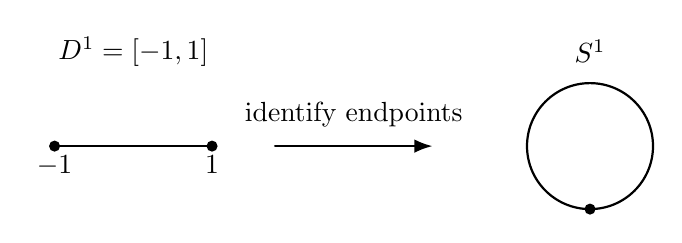
\begin{tikzpicture}[scale=1.0, >=Latex, line cap=round, line join=round]
		\begin{scope}[shift={(0,0)}]
			\node[font=\bfseries] at (0,1.2) {\(D^1=[-1,1]\)};
			\draw[thick] (-1,0) -- (1,0);
			\fill (-1,0) circle (2pt);
			\fill (1,0) circle (2pt);
			\node[below] at (-1,0) {\(-1\)};
			\node[below] at (1,0) {\(1\)};
		\end{scope}
		
		\draw[->, thick] (1.8,0) -- (3.8,0);
		\node[above] at (2.8,0.12) {identify endpoints};
		
		\begin{scope}[shift={(5.8,0)}]
			\node[font=\bfseries] at (0,1.2) {\(S^1\)};
			\draw[thick] (0,0) circle (0.8);
			\fill (0,-0.8) circle (2pt);
		\end{scope}
	\end{tikzpicture}
\end{center}

\subsubsection*{Case \(n=2\): \(D^2/S^1\cong S^2\)}

Here
\[
D^2=\{(x,y)\in\mathbb R^2:x^2+y^2\le 1\},
\qquad
S^1=\partial D^2.
\]
Thus we take the closed disk and collapse the entire boundary circle to a single point:
\[
D^2/S^1.
\]
The result is homeomorphic to the \(2\)-sphere:
\[
D^2/S^1\cong S^2.
\]

One may think of the interior of the disk as spreading across the sphere minus one point, while the whole boundary circle becomes that remaining point. Equivalently, a disk with boundary collapsed “closes up” into a sphere.

\begin{center}
	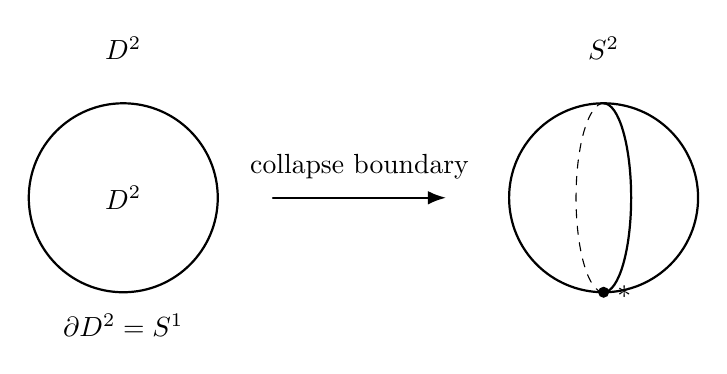
\begin{tikzpicture}[scale=1.0, >=Latex, line cap=round, line join=round]
		\begin{scope}[shift={(0,0)}]
			\node[font=\bfseries] at (0,1.9) {\(D^2\)};
			\draw[thick] (0,0) circle (1.2);
			\node at (0,0) {\(D^2\)};
			\node[below] at (0,-1.35) {\(\partial D^2=S^1\)};
		\end{scope}
		
		\draw[->, thick] (1.9,0) -- (4.1,0);
		\node[above] at (3,0.12) {collapse boundary};
		
		\begin{scope}[shift={(6.1,0)}]
			\node[font=\bfseries] at (0,1.9) {\(S^2\)};
			\draw[thick] (0,0) circle (1.2);
			\draw[thick] (0,-1.2) arc[start angle=-90,end angle=90,x radius=0.35,y radius=1.2];
			\draw[dashed] (0,-1.2) arc[start angle=-90,end angle=-270,x radius=0.35,y radius=1.2];
			\fill (0,-1.2) circle (2pt);
			\node[right] at (0.05,-1.2) {\(\ast\)};
		\end{scope}
	\end{tikzpicture}
\end{center}

\subsubsection*{Case \(n=3\): \(D^3/S^2\cong S^3\)}

Now
\[
D^3=\{(x,y,z)\in\mathbb R^3:x^2+y^2+z^2\le 1\},
\qquad
S^2=\partial D^3.
\]
We collapse the entire boundary \(2\)-sphere of the \(3\)-ball to one point:
\[
D^3/S^2.
\]
The resulting quotient is homeomorphic to the \(3\)-sphere:
\[
D^3/S^2\cong S^3.
\]

This is harder to visualize directly, but it is the exact higher-dimensional analogue of the previous cases. Just as an interval with endpoints identified gives a circle, and a disk with boundary circle collapsed gives a \(2\)-sphere, a \(3\)-ball with boundary \(2\)-sphere collapsed gives a \(3\)-sphere.

A useful intuition is that \(S^3\) may be viewed as two \(3\)-balls glued along their common boundary \(S^2\). If one keeps one \(3\)-ball and collapses its boundary to a point, one recovers the same space up to homeomorphism.

\begin{center}
	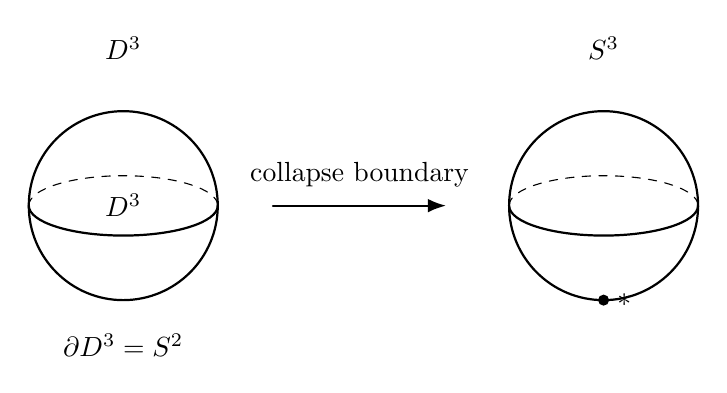
\begin{tikzpicture}[scale=1.0, >=Latex, line cap=round, line join=round]
		\begin{scope}[shift={(0,0)}]
			\node[font=\bfseries] at (0,2.0) {\(D^3\)};
			\draw[thick] (0,0) circle (1.2);
			\draw[thick] (-1.2,0) arc[start angle=180,end angle=360,x radius=1.2,y radius=0.38];
			\draw[dashed] (-1.2,0) arc[start angle=180,end angle=0,x radius=1.2,y radius=0.38];
			\node at (0,0) {\(D^3\)};
			\node[below] at (0,-1.5) {\(\partial D^3=S^2\)};
		\end{scope}
		
		\draw[->, thick] (1.9,0) -- (4.1,0);
		\node[above] at (3,0.12) {collapse boundary};
		
		\begin{scope}[shift={(6.1,0)}]
			\node[font=\bfseries] at (0,2.0) {\(S^3\)};
			\draw[thick] (0,0) circle (1.2);
			\draw[thick] (-1.2,0) arc[start angle=180,end angle=360,x radius=1.2,y radius=0.38];
			\draw[dashed] (-1.2,0) arc[start angle=180,end angle=0,x radius=1.2,y radius=0.38];
			\fill (0,-1.2) circle (2pt);
			\node[right] at (0.05,-1.2) {\(\ast\)};
		\end{scope}
	\end{tikzpicture}
\end{center}

\subsubsection*{Summary of the first three cases}

The pattern is:
\[
D^1/S^0\cong S^1,\qquad
D^2/S^1\cong S^2,\qquad
D^3/S^2\cong S^3.
\]
In each case, the whole boundary of the disk or ball is collapsed to one point, and the resulting quotient is a sphere.

This is the general rule:
\[
\boxed{D^n/S^{n-1}\cong S^n.}
\]

\medskip

\noindent
\textbf{Conceptual meaning.}
This quotient explains why an \(n\)-cell contributes one generator in dimension \(n\) to cellular homology. Relative to its boundary, a cell behaves exactly like a sphere:
\[
H_k(D^n,S^{n-1})\cong \widetilde H_k(S^n).
\]
Thus the quotient \(D^n/S^{n-1}\cong S^n\) is one of the central geometric facts behind the whole cellular chain complex.




\subsection{Concrete and deeper examples of the quotient \(D^n/S^{n-1}\cong S^n\)}

The quotient
\[
D^n/S^{n-1}\cong S^n
\]
is one of the most important constructions in algebraic topology. It appears in the theory of CW complexes, relative homology, one-point compactification, and the geometry of attaching cells. Although the statement is simple, it has many interpretations and many concrete models. In this subsection we present several examples, starting from the most elementary cases and moving toward deeper structural applications.

\subsubsection*{Example 1: the interval and the circle}

Let
\[
D^1=[-1,1],
\qquad
S^0=\{-1,1\}.
\]
Then
\[
D^1/S^0=[-1,1]/\{-1,1\},
\]
which means that the two endpoints of the interval are identified. The resulting space is homeomorphic to a circle:
\[
D^1/S^0\cong S^1.
\]

This is the simplest possible example of the general phenomenon. Geometrically, the interval has two boundary points, and once these boundary points are glued together, the interval closes into a loop. The interior \((-1,1)\) remains distinct, but the boundary becomes a single point in the quotient.

This example already contains the essential pattern of all higher-dimensional cases: the interior of the disk remains as the ``main body'' of the space, while the whole boundary is compressed into one single point, thereby producing a sphere.

\begin{center}
	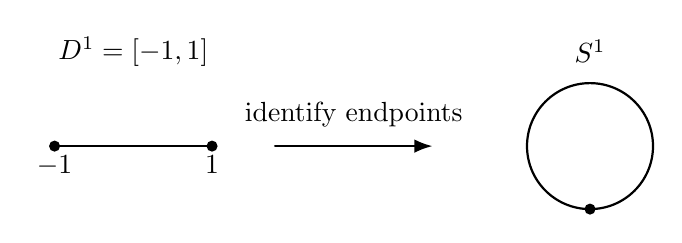
\begin{tikzpicture}[scale=1.0, >=Latex, line cap=round, line join=round]
		\begin{scope}[shift={(0,0)}]
			\node[font=\bfseries] at (0,1.2) {\(D^1=[-1,1]\)};
			\draw[thick] (-1,0) -- (1,0);
			\fill (-1,0) circle (2pt);
			\fill (1,0) circle (2pt);
			\node[below] at (-1,0) {\(-1\)};
			\node[below] at (1,0) {\(1\)};
		\end{scope}
		
		\draw[->, thick] (1.8,0) -- (3.8,0);
		\node[above] at (2.8,0.12) {identify endpoints};
		
		\begin{scope}[shift={(5.8,0)}]
			\node[font=\bfseries] at (0,1.2) {\(S^1\)};
			\draw[thick] (0,0) circle (0.8);
			\fill (0,-0.8) circle (2pt);
		\end{scope}
	\end{tikzpicture}
\end{center}

\subsubsection*{Example 2: the disk and the \(2\)-sphere}

Now let
\[
D^2=\{(x,y)\in \mathbb R^2:x^2+y^2\le 1\},
\qquad
S^1=\partial D^2.
\]
The quotient
\[
D^2/S^1
\]
is obtained by collapsing the entire boundary circle to one point. The result is homeomorphic to the \(2\)-sphere:
\[
D^2/S^1\cong S^2.
\]

This is one of the most useful examples in practice. One may think of the interior of the disk as spreading across the sphere minus one point, while the whole boundary circle becomes that missing point. In this sense the quotient ``closes up'' the disk into a sphere.

A closely related model is obtained from the square \(I^2=[0,1]^2\). Since \(I^2\) is homeomorphic to \(D^2\), one also has
\[
I^2/\partial I^2 \cong S^2.
\]
This version is often easier to visualize combinatorially: the interior of the square remains two-dimensional, while every edge and every corner is identified into one single point. The quotient is still a sphere.

\begin{center}
	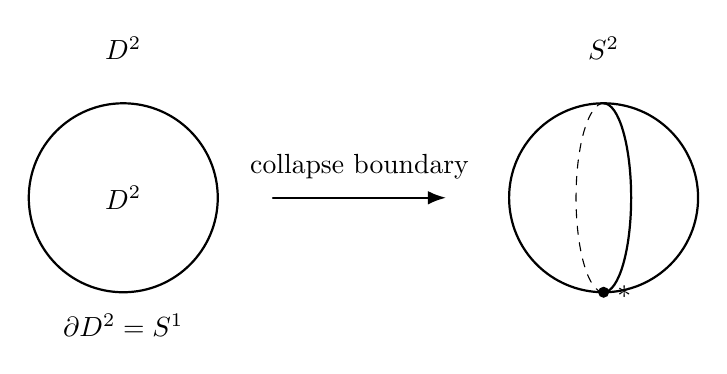
\begin{tikzpicture}[scale=1.0, >=Latex, line cap=round, line join=round]
		\begin{scope}[shift={(0,0)}]
			\node[font=\bfseries] at (0,1.9) {\(D^2\)};
			\draw[thick] (0,0) circle (1.2);
			\node at (0,0) {\(D^2\)};
			\node[below] at (0,-1.35) {\(\partial D^2=S^1\)};
		\end{scope}
		
		\draw[->, thick] (1.9,0) -- (4.1,0);
		\node[above] at (3,0.12) {collapse boundary};
		
		\begin{scope}[shift={(6.1,0)}]
			\node[font=\bfseries] at (0,1.9) {\(S^2\)};
			\draw[thick] (0,0) circle (1.2);
			\draw[thick] (0,-1.2) arc[start angle=-90,end angle=90,x radius=0.35,y radius=1.2];
			\draw[dashed] (0,-1.2) arc[start angle=-90,end angle=-270,x radius=0.35,y radius=1.2];
			\fill (0,-1.2) circle (2pt);
			\node[right] at (0.05,-1.2) {\(\ast\)};
		\end{scope}
	\end{tikzpicture}
\end{center}

\subsubsection*{Example 3: the \(3\)-ball and the \(3\)-sphere}

Let
\[
D^3=\{(x,y,z)\in\mathbb R^3:x^2+y^2+z^2\le 1\},
\qquad
S^2=\partial D^3.
\]
The quotient
\[
D^3/S^2
\]
collapses the entire boundary \(2\)-sphere to one point. The result is homeomorphic to the \(3\)-sphere:
\[
D^3/S^2\cong S^3.
\]

This case is harder to visualize directly, since \(S^3\) does not sit naturally inside ordinary \(\mathbb R^3\) as a visible surface. Nevertheless, it is the exact higher-dimensional analogue of the previous cases. Just as an interval with endpoints identified gives a circle, and a disk with boundary collapsed gives a \(2\)-sphere, a \(3\)-ball with boundary \(2\)-sphere collapsed gives a \(3\)-sphere.

A useful alternative model is the cube:
\[
I^3/\partial I^3\cong S^3.
\]
Again the precise shape does not matter. What matters topologically is that there is a \(3\)-dimensional interior and a \(2\)-dimensional boundary, and that the whole boundary is collapsed to a single point.

\begin{center}
	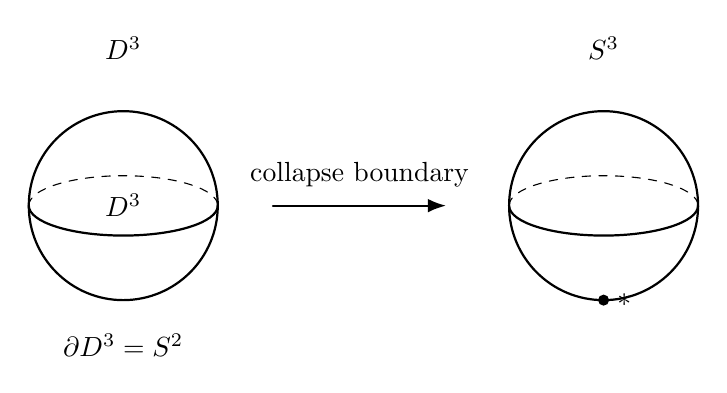
\begin{tikzpicture}[scale=1.0, >=Latex, line cap=round, line join=round]
		\begin{scope}[shift={(0,0)}]
			\node[font=\bfseries] at (0,2.0) {\(D^3\)};
			\draw[thick] (0,0) circle (1.2);
			\draw[thick] (-1.2,0) arc[start angle=180,end angle=360,x radius=1.2,y radius=0.38];
			\draw[dashed] (-1.2,0) arc[start angle=180,end angle=0,x radius=1.2,y radius=0.38];
			\node at (0,0) {\(D^3\)};
			\node[below] at (0,-1.5) {\(\partial D^3=S^2\)};
		\end{scope}
		
		\draw[->, thick] (1.9,0) -- (4.1,0);
		\node[above] at (3,0.12) {collapse boundary};
		
		\begin{scope}[shift={(6.1,0)}]
			\node[font=\bfseries] at (0,2.0) {\(S^3\)};
			\draw[thick] (0,0) circle (1.2);
			\draw[thick] (-1.2,0) arc[start angle=180,end angle=360,x radius=1.2,y radius=0.38];
			\draw[dashed] (-1.2,0) arc[start angle=180,end angle=0,x radius=1.2,y radius=0.38];
			\fill (0,-1.2) circle (2pt);
			\node[right] at (0.05,-1.2) {\(\ast\)};
		\end{scope}
	\end{tikzpicture}
\end{center}

\subsubsection*{Example 4: relative homology of a cell}

One of the deepest reasons this quotient is important is that it explains the relative homology of a disk modulo its boundary. In general, for a pair \((X,A)\), one has
\[
H_k(X,A)\cong \widetilde H_k(X/A).
\]
Applying this to
\[
X=D^n,
\qquad
A=S^{n-1},
\]
we obtain
\[
H_k(D^n,S^{n-1})
\cong
\widetilde H_k(D^n/S^{n-1})
\cong
\widetilde H_k(S^n).
\]
Therefore
\[
H_k(D^n,S^{n-1})\cong
\begin{cases}
	\mathbb Z, & k=n,\\
	0, & k\neq n.
\end{cases}
\]

This is an extremely important fact. It says that an \(n\)-cell, viewed relative to its boundary, behaves exactly like an \(n\)-sphere. In other words, once the boundary has been collapsed away, the essential homological content of the cell is a single generator in dimension \(n\).

This fact is one of the foundations of cellular homology.

\subsubsection*{Example 5: why CW complexes lead to wedges of spheres}

Let \(X\) be a CW complex and let \(X^n\) denote its \(n\)-skeleton. The quotient
\[
X^n/X^{n-1}
\]
is obtained by collapsing the entire \((n-1)\)-skeleton to a point. Each \(n\)-cell \(e_\alpha^n\) is a copy of \(D^n\) attached along its boundary \(S^{n-1}\) to the lower skeleton. Once \(X^{n-1}\) is collapsed, the boundary of each cell is also collapsed, so each cell becomes
\[
D^n/S^{n-1}\cong S^n.
\]
Therefore
\[
X^n/X^{n-1}\cong \bigvee_{\alpha\in I_n} S^n,
\]
a wedge of \(n\)-spheres, one for each \(n\)-cell of \(X\).

This is one of the deepest and most useful applications of the quotient \(D^n/S^{n-1}\cong S^n\). It explains why
\[
H_k(X^n,X^{n-1})\cong
\begin{cases}
	\mathbb Z^{r_n}, & k=n,\\
	0, & k\neq n,
\end{cases}
\]
where \(r_n\) is the number of \(n\)-cells. Thus the cellular chain group
\[
C_n^{\mathrm{cell}}(X)=H_n(X^n,X^{n-1})
\]
is free abelian on the \(n\)-cells.

So the simple geometric quotient \(D^n/S^{n-1}\cong S^n\) is not just an isolated fact: it is a structural reason why cellular homology works at all.

\subsubsection*{Example 6: spheres as two disks glued together}

Another very useful viewpoint comes from decomposing the sphere into two hemispheres:
\[
S^n = D^n_+ \cup D^n_-,
\qquad
D^n_+ \cap D^n_- = S^{n-1}.
\]
Thus a sphere may be built by gluing two \(n\)-disks along their common boundary.

Now look at only one hemisphere, say \(D^n_+\). If its boundary \(S^{n-1}\) is collapsed to a point, then one obtains the whole sphere:
\[
D^n/S^{n-1}\cong S^n.
\]
This interpretation is especially valuable geometrically: one disk already contains all the interior data, and collapsing its boundary supplies the additional point needed to complete the sphere.

So the quotient construction is closely related to the idea that a sphere is a compactification of Euclidean space.

\subsubsection*{Example 7: one-point compactification of \(\mathbb R^n\)}

The interior of the disk \(D^n\) is homeomorphic to \(\mathbb R^n\). When the boundary \(S^{n-1}\) is collapsed to one point, one is essentially adding one point ``at infinity'' to \(\mathbb R^n\). The resulting compact space is the one-point compactification of \(\mathbb R^n\), namely
\[
\mathbb R^n\cup\{\infty\}\cong S^n.
\]

This gives a deeper interpretation of the quotient:
\[
D^n/S^{n-1}\cong S^n
\]
may be viewed as a compactification statement. The whole boundary sphere is compressed into a single point, and that point plays the role of infinity.

This viewpoint is fundamental in many areas of topology, geometry, and analysis. It connects Euclidean space, spheres, and quotient spaces in a single picture.

\subsubsection*{Example 8: the top cell in projective space}

Real projective space \(\mathbb{RP}^n\) has a CW structure with exactly one cell in each dimension \(0,1,\dots,n\). The top quotient
\[
\mathbb{RP}^n/\mathbb{RP}^{n-1}
\]
collapses the lower skeleton to a point, leaving only the top \(n\)-cell modulo its boundary. Therefore
\[
\mathbb{RP}^n/\mathbb{RP}^{n-1}\cong D^n/S^{n-1}\cong S^n.
\]

This is a strong structural example. It shows that the quotient \(D^n/S^{n-1}\cong S^n\) is not merely about isolated disks and balls; it appears naturally inside major spaces built by cells. It is one of the recurring geometric patterns behind filtrations and skeletal quotients.

\subsubsection*{Conceptual summary}

These examples all express the same central principle:
\[
\boxed{\text{an \(n\)-cell, after collapsing its boundary, becomes an \(n\)-sphere}.}
\]

In dimension \(1\), this means identifying the endpoints of an interval. In dimension \(2\), it means collapsing the boundary circle of a disk. In dimension \(3\), it means collapsing the boundary sphere of a ball. In CW theory, it means that each cell contributes a sphere to the quotient \(X^n/X^{n-1}\). In relative homology, it means that the pair \((D^n,S^{n-1})\) behaves exactly like \(S^n\).

Thus the quotient
\[
D^n/S^{n-1}\cong S^n
\]
is not merely a computational trick. It is one of the central geometric facts that connects quotient spaces, cells, spheres, relative homology, and the whole architecture of CW complexes.

\section{Problem 6. Realizing a homology class by a finite cell complex}

\textbf{Problem.} Suppose \(x\in H_n(X)\), where \(X\) is an arbitrary topological space. Show that there is a finite cell complex \(A\) and a map
\[
f:A\to X
\]
such that
\[
x\in \operatorname{im}\bigl(f_*:H_n(A)\to H_n(X)\bigr).
\]

\medskip

\textbf{Solution.}
Choose a singular cycle \(z\in Z_n(X)\) representing the class \(x\). Since singular chains are finite sums, we may write
\[
z=\sum_{i=1}^r a_i\sigma_i,
\]
where each \(\sigma_i:\Delta^n\to X\) is a singular \(n\)-simplex and each \(a_i\in \mathbb Z\).

We now replace each coefficient \(a_i\) by repeated copies of the corresponding simplex, reversing orientation when \(a_i<0\). Thus we may think of \(z\) as a finite sum
\[
z=\sum_{j=1}^N \varepsilon_j \sigma_j,
\qquad \varepsilon_j\in\{+1,-1\},
\]
of finitely many oriented singular \(n\)-simplices.

For each \(\sigma_j\), take a copy \(\Delta_j^n\) of the standard \(n\)-simplex. Since \(\partial z=0\), each oriented \((n-1)\)-face appearing in the boundary occurs with total coefficient zero. In particular, the faces can be paired so that whenever two faces are paired, the corresponding singular \((n-1)\)-simplices in \(X\) agree, but with opposite induced orientations.

We now glue the copies \(\Delta_j^n\) along these paired boundary faces. Because only finitely many simplices are involved, the resulting space \(A\) is a finite \(\Delta\)-complex, hence in particular a finite cell complex.

The singular maps \(\sigma_j:\Delta_j^n\to X\) fit together under these identifications, precisely because paired faces map to the same singular \((n-1)\)-simplex in \(X\). Therefore they descend to a continuous map
\[
f:A\to X.
\]

Let \(c_A\) denote the sum of the top-dimensional simplices of \(A\) with the induced orientations. By construction, the boundary faces cancel in pairs, so
\[
\partial c_A=0.
\]
Hence \(c_A\) defines a homology class
\[
[c_A]\in H_n(A).
\]
Moreover, by construction,
\[
f_*([c_A])=[z]=x.
\]
Therefore
\[
x\in \operatorname{im}(f_*).
\]

\medskip

Thus every homology class in \(H_n(X)\) is realized by a map from a finite cell complex.

\bigskip

\section{Problem 7. Cellular maps and cellular chain complexes}

\textbf{Problem.} Let \(X\) and \(Y\) be finite cell complexes. A map
\[
f:X\to Y
\]
is called \emph{cellular} if \(f(X_n)\subseteq Y_n\) for all \(n\), where \(X_n\) and \(Y_n\) denote the \(n\)-skeleta. Show that such a map induces a chain map
\[
f_*^{\mathrm{cell}}:C_*^{\mathrm{cell}}(X)\to C_*^{\mathrm{cell}}(Y),
\]
and that the induced map on homology agrees with the usual map
\[
f_*:H_*(X)\to H_*(Y).
\]

\medskip

\textbf{Solution.}
Recall that the cellular chain groups are defined by
\[
C_n^{\mathrm{cell}}(X)=H_n(X_n,X_{n-1}),
\qquad
C_n^{\mathrm{cell}}(Y)=H_n(Y_n,Y_{n-1}).
\]

Since \(f\) is cellular, for every \(n\) we have
\[
f(X_n)\subseteq Y_n
\qquad\text{and}\qquad
f(X_{n-1})\subseteq Y_{n-1}.
\]
Hence \(f\) induces a map of pairs
\[
f:(X_n,X_{n-1})\to (Y_n,Y_{n-1}),
\]
and therefore a homomorphism
\[
f_n^{\mathrm{cell}}:
H_n(X_n,X_{n-1})\longrightarrow H_n(Y_n,Y_{n-1}).
\]
So for each \(n\) we obtain a map
\[
f_n^{\mathrm{cell}}:C_n^{\mathrm{cell}}(X)\to C_n^{\mathrm{cell}}(Y).
\]

It remains to verify that these maps commute with the cellular boundary operators. The cellular differential
\[
d_n:C_n^{\mathrm{cell}}(X)\to C_{n-1}^{\mathrm{cell}}(X)
\]
is defined using the connecting homomorphisms in the long exact sequence of the triple
\[
(X_n,X_{n-1},X_{n-2}),
\]
and similarly for \(Y\). Since \(f\) preserves skeleta, it induces a map of triples
\[
(X_n,X_{n-1},X_{n-2})\to (Y_n,Y_{n-1},Y_{n-2}).
\]
By naturality of the connecting homomorphism, we obtain
\[
d_n\circ f_n^{\mathrm{cell}}
=
f_{n-1}^{\mathrm{cell}}\circ d_n.
\]
Thus
\[
f_*^{\mathrm{cell}}:C_*^{\mathrm{cell}}(X)\to C_*^{\mathrm{cell}}(Y)
\]
is a chain map.

We now compare the induced map on homology with the usual singular-homology map. For CW complexes, cellular homology is naturally isomorphic to singular homology:
\[
H_*^{\mathrm{cell}}(X)\cong H_*(X),
\qquad
H_*^{\mathrm{cell}}(Y)\cong H_*(Y).
\]
These isomorphisms are natural with respect to cellular maps. Consequently, under the canonical identifications
\[
H_*^{\mathrm{cell}}(X)\cong H_*(X),
\qquad
H_*^{\mathrm{cell}}(Y)\cong H_*(Y),
\]
the homomorphism induced by the cellular chain map \(f_*^{\mathrm{cell}}\) agrees exactly with the usual map
\[
f_*:H_*(X)\to H_*(Y).
\]

\medskip

Therefore a cellular map induces a cellular chain map, and its induced map on homology is the same as the standard homology map.

\bigskip

\section{Problem 8. The quotient map for \(X=S^n\cup_f D^{n+1}\)}

\textbf{Problem.} Let
\[
f:S^n\to S^n
\]
have degree \(k\), and let
\[
X=S^n\cup_f D^{n+1}.
\]
Let
\[
\pi:X\to X/S^n\cong S^{n+1}
\]
be the quotient map. Compute
\[
\pi^*:H^*(S^{n+1})\to H^*(X)
\qquad\text{and}\qquad
\pi_*:H_*(X)\to H_*(S^{n+1}).
\]

\medskip

\textbf{Solution.}
The space \(X\) has a CW structure with one \(0\)-cell, one \(n\)-cell, and one \((n+1)\)-cell. The attaching map of the \((n+1)\)-cell has degree \(k\), so the cellular chain complex of \(X\) is
\[
0\longrightarrow C_{n+1}^{\mathrm{cell}}(X)\cong \mathbb Z
\xrightarrow{\ \times k\ }
C_n^{\mathrm{cell}}(X)\cong \mathbb Z
\longrightarrow 0,
\]
together with \(C_0^{\mathrm{cell}}(X)\cong \mathbb Z\).

Hence
\[
H_{n+1}(X)=\ker(\times k:\mathbb Z\to\mathbb Z),
\qquad
H_n(X)=\operatorname{coker}(\times k:\mathbb Z\to\mathbb Z)\cong \mathbb Z/k\mathbb Z.
\]
So, if \(k\neq 0\), then
\[
H_{n+1}(X)=0,
\qquad
H_n(X)\cong \mathbb Z/k\mathbb Z,
\qquad
H_0(X)\cong \mathbb Z,
\]
and all other homology groups vanish. If \(k=0\), then
\[
H_{n+1}(X)\cong \mathbb Z,
\qquad
H_n(X)\cong \mathbb Z,
\]
so in that case \(X\simeq S^n\vee S^{n+1}\).

Dually, the cellular cochain complex gives
\[
H^{n+1}(X)\cong \operatorname{coker}(\times k:\mathbb Z\to\mathbb Z)\cong \mathbb Z/k\mathbb Z,
\qquad
H^n(X)\cong \ker(\times k:\mathbb Z\to\mathbb Z),
\]
and therefore, for \(k\neq 0\),
\[
H^{n+1}(X)\cong \mathbb Z/k\mathbb Z,
\qquad
H^n(X)=0,
\qquad
H^0(X)\cong \mathbb Z.
\]

Now collapse the subspace \(S^n\subset X\). Since \(X\) is obtained from \(S^n\) by attaching one \((n+1)\)-cell, we have
\[
X/S^n\cong S^{n+1}.
\]
Moreover,
\[
\widetilde H_*(X/S^n)\cong H_*(X,S^n),
\qquad
\widetilde H^*(X/S^n)\cong H^*(X,S^n),
\]
and under these identifications the quotient map \(\pi\) corresponds to the canonical passage from absolute groups to relative groups.

\medskip

\textbf{Computation of \(\pi_*\).}
Consider the long exact sequence of the pair \((X,S^n)\):
\[
0\to H_{n+1}(X)\to H_{n+1}(X,S^n)\xrightarrow{\partial} H_n(S^n)\to H_n(X)\to 0.
\]
Since
\[
H_{n+1}(X,S^n)\cong \widetilde H_{n+1}(X/S^n)\cong H_{n+1}(S^{n+1})\cong \mathbb Z,
\]
and the connecting homomorphism \(\partial\) is multiplication by \(k\), it follows that
\[
H_{n+1}(X)=\ker(\times k:\mathbb Z\to\mathbb Z).
\]
The map
\[
\pi_*:H_{n+1}(X)\to H_{n+1}(S^{n+1})\cong \mathbb Z
\]
is precisely the inclusion of this kernel into \(\mathbb Z\). Therefore:
\[
\pi_*=
\begin{cases}
	\mathrm{id}_{\mathbb Z}, & *=0,\\[1mm]
	0, & *=n+1 \text{ and } k\neq 0,\\[1mm]
	\text{an isomorphism }\mathbb Z\to\mathbb Z, & *=n+1 \text{ and } k=0,\\[1mm]
	0, & \text{in all other positive degrees.}
\end{cases}
\]

\medskip

\textbf{Computation of \(\pi^*\).}
Now use the long exact sequence in cohomology:
\[
0\to H^n(X)\to H^n(S^n)\xrightarrow{\delta} H^{n+1}(X,S^n)\to H^{n+1}(X)\to 0.
\]
Again,
\[
H^{n+1}(X,S^n)\cong \widetilde H^{n+1}(X/S^n)\cong H^{n+1}(S^{n+1})\cong \mathbb Z,
\]
and the connecting map \(\delta\) is multiplication by \(k\). Hence
\[
H^{n+1}(X)\cong \mathbb Z/k\mathbb Z.
\]
Under the identification \(H^{n+1}(X,S^n)\cong H^{n+1}(S^{n+1})\), the map
\[
\pi^*:H^{n+1}(S^{n+1})\to H^{n+1}(X)
\]
is exactly the quotient map
\[
\mathbb Z\to \mathbb Z/k\mathbb Z,
\qquad
m\mapsto \overline{m}.
\]
Thus
\[
\pi^*=
\begin{cases}
	\mathrm{id}_{\mathbb Z}, & *=0,\\[1mm]
	\mathbb Z\to \mathbb Z/k\mathbb Z,\quad m\mapsto \overline{m}, & *=n+1 \text{ and } k\neq 0,\\[1mm]
	\text{an isomorphism }\mathbb Z\to\mathbb Z, & *=n+1 \text{ and } k=0,\\[1mm]
	0, & \text{in all other degrees.}
\end{cases}
\]

\medskip

In particular, for \(k\neq 0\), the quotient map \(\pi\) is trivial on positive-dimensional homology, but in cohomology it sends a generator of \(H^{n+1}(S^{n+1})\cong \mathbb Z\) to the generator of
\[
H^{n+1}(X)\cong \mathbb Z/k\mathbb Z
\]
modulo \(k\).

\bigskip

\noindent
\textbf{Summary.}
These three problems illustrate three central themes in algebraic topology:

\begin{itemize}
	\item every homology class is represented by a map from a finite cell complex;
	\item cellular maps act directly on cellular chain complexes and recover the usual maps on homology;
	\item attaching maps of spheres control the algebraic structure of the resulting space, and quotient maps detect this structure naturally in homology and cohomology.
\end{itemize}

\section{Problem 9. Compatibility of boundary maps with the Kronecker pairing}

\textbf{Statement.}
Let
\[
\partial : H_*(X,A)\longrightarrow H_{*-1}(A)
\]
and
\[
\delta : H^*(A)\longrightarrow H^{*+1}(X,A)
\]
be the boundary maps in the long exact homology and cohomology sequences of the pair \((X,A)\). If
\[
a\in H^k(A)
\qquad\text{and}\qquad
x\in H_{k+1}(X,A),
\]
show that
\[
\langle a,\partial x\rangle=\langle \delta a,x\rangle .
\]

\medskip

\textbf{Solution.}
We prove the identity directly from the chain-level definitions of the connecting homomorphisms.

Let
\[
\alpha\in Z^k(A)
\]
be a cocycle representing the cohomology class \(a\in H^k(A)\). Also let
\[
c\in C_{k+1}(X)
\]
be a singular chain representing the relative homology class
\[
x\in H_{k+1}(X,A).
\]
Since \(c\) represents a relative cycle, its boundary lies in \(A\), that is,
\[
\partial c\in C_k(A).
\]
Therefore the homology boundary \(\partial x\in H_k(A)\) is represented by the cycle \(\partial c\).

Hence
\[
\langle a,\partial x\rangle
=
\alpha(\partial c).
\]

Now we describe the cohomology connecting homomorphism. Choose a cochain
\[
\widetilde{\alpha}\in C^k(X)
\]
extending \(\alpha\), meaning that
\[
\widetilde{\alpha}|_{C_k(A)}=\alpha.
\]
Because \(\alpha\) is a cocycle on \(A\), we have
\[
d\alpha=0.
\]
Thus \(d\widetilde{\alpha}\) vanishes on \(C_{k+1}(A)\), so it defines a relative cocycle
\[
d\widetilde{\alpha}\in Z^{k+1}(X,A).
\]
By definition of the connecting homomorphism in cohomology,
\[
\delta a=[d\widetilde{\alpha}]\in H^{k+1}(X,A).
\]

Therefore
\[
\langle \delta a,x\rangle
=
(d\widetilde{\alpha})(c).
\]
Using the definition of the coboundary,
\[
(d\widetilde{\alpha})(c)
=
\widetilde{\alpha}(\partial c).
\]
But \(\partial c\in C_k(A)\), and \(\widetilde{\alpha}\) restricts to \(\alpha\) on \(A\). Hence
\[
\widetilde{\alpha}(\partial c)
=
\alpha(\partial c).
\]
Thus
\[
\langle \delta a,x\rangle
=
\alpha(\partial c)
=
\langle a,\partial x\rangle.
\]

Therefore
\[
\boxed{
	\langle a,\partial x\rangle=\langle \delta a,x\rangle .
}
\]

\medskip

\textbf{Remark.}
The proof says that the following square is compatible with the natural pairing:
\[
\begin{array}{ccc}
	H^k(A)\times H_{k+1}(X,A) & \longrightarrow & \mathbb Z \\[1mm]
	\delta\times \mathrm{id}\downarrow\phantom{\delta\times \mathrm{id}} 
	&& 
	\phantom{\mathrm{id}\times \partial}\downarrow \mathrm{id} \\[1mm]
	H^{k+1}(X,A)\times H_{k+1}(X,A) & \longrightarrow & \mathbb Z ,
\end{array}
\]
or more concretely,
\[
\boxed{
	\text{evaluate first and then take a boundary}
	=
	\text{take a coboundary first and then evaluate.}
}
\]

\bigskip

\section{Problem 10. Coefficient short exact sequences and the Bockstein homomorphism}

\textbf{Statement.}
Suppose
\[
0\longrightarrow K\longrightarrow G\longrightarrow H\longrightarrow 0
\]
is a short exact sequence of abelian groups. If \(X\) is a space, show that there is a short exact sequence
\[
0\longrightarrow C_*(X;K)\longrightarrow C_*(X;G)\longrightarrow C_*(X;H)\longrightarrow 0.
\]

Let
\[
\beta_X:H_*(X;H)\longrightarrow H_{*-1}(X;K)
\]
be the boundary map in the associated long exact sequence. This map is called the \emph{Bockstein homomorphism}. If
\[
f:X\longrightarrow Y
\]
is a map, show that
\[
f_*\beta_X=\beta_Y f_*.
\]
If \(X=Y=\mathbb{RP}^n\), deduce that
\[
f_*:H_*(\mathbb{RP}^n;\mathbb Z/2)
\longrightarrow
H_*(\mathbb{RP}^n;\mathbb Z/2)
\]
is determined by
\[
f_*:H_*(\mathbb{RP}^n;\mathbb Z)
\longrightarrow
H_*(\mathbb{RP}^n;\mathbb Z).
\]
Show that the converse holds if \(n\) is even, but not if \(n\) is odd.

\medskip

\textbf{Solution.}

\subsection*{Step 1. The short exact sequence of chain complexes}

For singular chains with coefficients in an abelian group \(G\), we have
\[
C_n(X;G)=C_n(X)\otimes G.
\]
The group \(C_n(X)\) is a free abelian group, generated by all singular \(n\)-simplices in \(X\). Since tensoring with a free abelian group preserves short exact sequences, the short exact sequence
\[
0\longrightarrow K\longrightarrow G\longrightarrow H\longrightarrow 0
\]
gives, for every \(n\),
\[
0\longrightarrow C_n(X)\otimes K
\longrightarrow C_n(X)\otimes G
\longrightarrow C_n(X)\otimes H
\longrightarrow 0.
\]
Equivalently,
\[
0\longrightarrow C_n(X;K)
\longrightarrow C_n(X;G)
\longrightarrow C_n(X;H)
\longrightarrow 0.
\]

The maps commute with the boundary operators because the boundary with coefficients is given by
\[
\partial\otimes \mathrm{id}.
\]
Therefore the degreewise short exact sequences assemble into a short exact sequence of chain complexes:
\[
\boxed{
	0\longrightarrow C_*(X;K)
	\longrightarrow C_*(X;G)
	\longrightarrow C_*(X;H)
	\longrightarrow 0.
}
\]

\subsection*{Step 2. The Bockstein homomorphism}

From the short exact sequence of chain complexes
\[
0\longrightarrow C_*(X;K)
\longrightarrow C_*(X;G)
\longrightarrow C_*(X;H)
\longrightarrow 0,
\]
we obtain a long exact sequence in homology:
\[
\cdots
\longrightarrow
H_q(X;K)
\longrightarrow
H_q(X;G)
\longrightarrow
H_q(X;H)
\xrightarrow{\beta_X}
H_{q-1}(X;K)
\longrightarrow
H_{q-1}(X;G)
\longrightarrow
\cdots .
\]
The connecting homomorphism
\[
\beta_X:H_q(X;H)\longrightarrow H_{q-1}(X;K)
\]
is the Bockstein homomorphism associated with the coefficient sequence
\[
0\longrightarrow K\longrightarrow G\longrightarrow H\longrightarrow 0.
\]

\subsection*{Step 3. Naturality of the Bockstein homomorphism}

Let
\[
f:X\longrightarrow Y
\]
be a continuous map. It induces chain maps
\[
f_\#:C_*(X;K)\longrightarrow C_*(Y;K),
\]
\[
f_\#:C_*(X;G)\longrightarrow C_*(Y;G),
\]
and
\[
f_\#:C_*(X;H)\longrightarrow C_*(Y;H).
\]
These maps fit into a commutative diagram of short exact sequences of chain complexes:
\[
\begin{array}{ccccccccc}
	0 &\longrightarrow& C_*(X;K) &\longrightarrow& C_*(X;G) &\longrightarrow& C_*(X;H) &\longrightarrow& 0 \\[1mm]
	&& \downarrow f_\# && \downarrow f_\# && \downarrow f_\# && \\[1mm]
	0 &\longrightarrow& C_*(Y;K) &\longrightarrow& C_*(Y;G) &\longrightarrow& C_*(Y;H) &\longrightarrow& 0 .
\end{array}
\]
Passing to homology gives a commutative diagram of long exact sequences. In particular, the connecting homomorphisms commute with the maps induced by \(f\). Hence
\[
\boxed{
	f_*\beta_X=\beta_Y f_*.
}
\]

This is the naturality of the Bockstein homomorphism.

\subsection*{Step 4. The coefficient sequence for \(\mathbb{Z}/2\)}

Now take the standard short exact sequence
\[
0\longrightarrow \mathbb Z
\xrightarrow{\times 2}
\mathbb Z
\longrightarrow
\mathbb Z/2
\longrightarrow 0.
\]
The associated Bockstein homomorphism is
\[
\beta:
H_q(X;\mathbb Z/2)
\longrightarrow
H_{q-1}(X;\mathbb Z).
\]

For \(X=\mathbb{RP}^n\), the integral homology groups are
\[
H_q(\mathbb{RP}^n;\mathbb Z)
\cong
\begin{cases}
	\mathbb Z, & q=0,\\[1mm]
	\mathbb Z/2, & q \text{ odd and } 0<q<n,\\[1mm]
	\mathbb Z, & q=n \text{ and } n \text{ odd},\\[1mm]
	0, & \text{otherwise}.
\end{cases}
\]
The mod \(2\) homology groups are
\[
H_q(\mathbb{RP}^n;\mathbb Z/2)
\cong
\mathbb Z/2
\qquad
\text{for }0\le q\le n.
\]

The long exact coefficient sequence is
\[
\cdots
\longrightarrow
H_q(\mathbb{RP}^n;\mathbb Z)
\xrightarrow{\times 2}
H_q(\mathbb{RP}^n;\mathbb Z)
\longrightarrow
H_q(\mathbb{RP}^n;\mathbb Z/2)
\xrightarrow{\beta}
H_{q-1}(\mathbb{RP}^n;\mathbb Z)
\xrightarrow{\times 2}
H_{q-1}(\mathbb{RP}^n;\mathbb Z)
\longrightarrow
\cdots .
\]

\subsection*{Step 5. Why the integral map determines the mod \(2\) map}

We analyze degree by degree.

\medskip

\textbf{Case 1: \(q=0\).}
Since \(\mathbb{RP}^n\) is connected, every self-map
\[
f:\mathbb{RP}^n\longrightarrow \mathbb{RP}^n
\]
induces the identity map on \(H_0\), both with integral and mod \(2\) coefficients. Thus the mod \(2\) map in degree \(0\) is determined.

\medskip

\textbf{Case 2: \(q\) odd and \(0<q<n\).}
Then
\[
H_q(\mathbb{RP}^n;\mathbb Z)\cong \mathbb Z/2
\]
and
\[
H_{q-1}(\mathbb{RP}^n;\mathbb Z)=0.
\]
Therefore the reduction map
\[
H_q(\mathbb{RP}^n;\mathbb Z)
\longrightarrow
H_q(\mathbb{RP}^n;\mathbb Z/2)
\]
is an isomorphism. Hence the action of \(f_*\) on
\[
H_q(\mathbb{RP}^n;\mathbb Z/2)
\]
is determined by its action on
\[
H_q(\mathbb{RP}^n;\mathbb Z).
\]

\medskip

\textbf{Case 3: \(q\) even and \(0<q\le n\).}
Then
\[
H_q(\mathbb{RP}^n;\mathbb Z)=0
\]
and
\[
H_{q-1}(\mathbb{RP}^n;\mathbb Z)\cong \mathbb Z/2.
\]
The Bockstein map
\[
\beta:
H_q(\mathbb{RP}^n;\mathbb Z/2)
\longrightarrow
H_{q-1}(\mathbb{RP}^n;\mathbb Z)
\]
is an isomorphism. Since the Bockstein is natural, we have
\[
f_*\beta=\beta f_*.
\]
Therefore, because \(\beta\) is an isomorphism, the action of \(f_*\) on
\[
H_q(\mathbb{RP}^n;\mathbb Z/2)
\]
is determined by the action of \(f_*\) on
\[
H_{q-1}(\mathbb{RP}^n;\mathbb Z).
\]

\medskip

\textbf{Case 4: \(q=n\) and \(n\) is odd.}
Then
\[
H_n(\mathbb{RP}^n;\mathbb Z)\cong \mathbb Z
\]
and
\[
H_n(\mathbb{RP}^n;\mathbb Z/2)\cong \mathbb Z/2.
\]
The reduction map
\[
H_n(\mathbb{RP}^n;\mathbb Z)
\longrightarrow
H_n(\mathbb{RP}^n;\mathbb Z/2)
\]
sends an integer degree to its value modulo \(2\). Therefore the integral map on top homology determines the mod \(2\) map on top homology.

Combining all cases, we conclude that
\[
\boxed{
	f_*:H_*(\mathbb{RP}^n;\mathbb Z/2)
	\longrightarrow
	H_*(\mathbb{RP}^n;\mathbb Z/2)
}
\]
is determined by
\[
\boxed{
	f_*:H_*(\mathbb{RP}^n;\mathbb Z)
	\longrightarrow
	H_*(\mathbb{RP}^n;\mathbb Z).
}
\]

\subsection*{Step 6. The converse when \(n\) is even}

Assume now that \(n\) is even. Then
\[
H_q(\mathbb{RP}^n;\mathbb Z)
\cong
\begin{cases}
	\mathbb Z, & q=0,\\[1mm]
	\mathbb Z/2, & q \text{ odd and }0<q<n,\\[1mm]
	0, & \text{otherwise}.
\end{cases}
\]
For every odd \(q\) with \(0<q<n\), the reduction map
\[
H_q(\mathbb{RP}^n;\mathbb Z)
\longrightarrow
H_q(\mathbb{RP}^n;\mathbb Z/2)
\]
is an isomorphism. Therefore the mod \(2\) map determines the integral map in all nonzero positive degrees.

In degree \(0\), since \(\mathbb{RP}^n\) is connected, every self-map induces the identity map on
\[
H_0(\mathbb{RP}^n;\mathbb Z)\cong \mathbb Z.
\]
Thus degree \(0\) is also determined.

Therefore, when \(n\) is even, the mod \(2\) homology action determines the integral homology action. Hence
\[
\boxed{
	\text{if }n\text{ is even, the converse holds.}
}
\]

\subsection*{Step 7. Failure of the converse when \(n\) is odd}

Now assume \(n\) is odd. Then \(\mathbb{RP}^n\) is orientable and
\[
H_n(\mathbb{RP}^n;\mathbb Z)\cong \mathbb Z.
\]
The mod \(2\) homology group in top degree is only
\[
H_n(\mathbb{RP}^n;\mathbb Z/2)\cong \mathbb Z/2.
\]
Thus mod \(2\) homology cannot distinguish multiplication by \(+1\) from multiplication by \(-1\) on the top integral homology group.

Indeed, compare the identity map
\[
\mathrm{id}:\mathbb{RP}^n\longrightarrow \mathbb{RP}^n
\]
with the projective linear homeomorphism induced by the reflection
\[
(x_0,x_1,\dots,x_n)\longmapsto (-x_0,x_1,\dots,x_n).
\]
This reflection has determinant \(-1\). Since \(n\) is odd, \(\mathbb{RP}^n\) is orientable, and the induced map on top homology is multiplication by \(-1\):
\[
r_*=-\mathrm{id}
\qquad
\text{on }
H_n(\mathbb{RP}^n;\mathbb Z)\cong \mathbb Z.
\]
By contrast, the identity map induces multiplication by \(+1\) on
\[
H_n(\mathbb{RP}^n;\mathbb Z).
\]
Therefore the two maps induce different maps on integral homology.

However, with \(\mathbb Z/2\)-coefficients, we have
\[
+1=-1
\qquad
\text{in }
\mathbb Z/2.
\]
So these two maps induce the same map on
\[
H_n(\mathbb{RP}^n;\mathbb Z/2).
\]
In fact, since each group
\[
H_q(\mathbb{RP}^n;\mathbb Z/2)
\]
is either \(0\) or \(\mathbb Z/2\), and since a homeomorphism induces an isomorphism in homology, it must induce the identity on each nonzero mod \(2\) homology group.

Thus the identity map and the orientation-reversing projective homeomorphism have the same action on mod \(2\) homology but different actions on integral homology.

Therefore
\[
\boxed{
	\text{if }n\text{ is odd, the converse does not hold.}
}
\]

\subsection*{Summary}

For the coefficient sequence
\[
0\longrightarrow \mathbb Z
\xrightarrow{\times 2}
\mathbb Z
\longrightarrow
\mathbb Z/2
\longrightarrow 0,
\]
the associated Bockstein homomorphism is natural:
\[
\boxed{
	f_*\beta_X=\beta_Y f_*.
}
\]
For \(X=Y=\mathbb{RP}^n\), this naturality implies that the integral homology action determines the mod \(2\) homology action:
\[
\boxed{
	f_* \text{ on } H_*(\mathbb{RP}^n;\mathbb Z)
	\quad\Longrightarrow\quad
	f_* \text{ on } H_*(\mathbb{RP}^n;\mathbb Z/2).
}
\]
The converse holds when \(n\) is even, because there is no top-dimensional infinite cyclic homology group. It fails when \(n\) is odd, because the top homology group is
\[
H_n(\mathbb{RP}^n;\mathbb Z)\cong \mathbb Z,
\]
and mod \(2\) homology cannot distinguish the maps \(+1\) and \(-1\) on this group.

\section{Theory for Problems 9--10: Pairings, boundary maps, coefficient sequences, and the Bockstein homomorphism}

\subsection{Relative chain complexes and the long exact homology sequence}

Let \(A\subseteq X\) be a subspace. The singular chain groups of \(X\) and \(A\) fit into a short exact sequence of chain complexes
\[
0
\longrightarrow
C_*(A)
\longrightarrow
C_*(X)
\longrightarrow
C_*(X,A)
\longrightarrow
0,
\]
where
\[
C_n(X,A)=C_n(X)/C_n(A).
\]
Thus an element of \(C_n(X,A)\) is represented by an \(n\)-chain in \(X\), where two chains are considered the same if their difference lies entirely in \(A\).

The boundary map on relative chains is induced from the usual boundary map on \(C_*(X)\). If a chain
\[
c\in C_n(X)
\]
represents a relative cycle in \(C_n(X,A)\), then
\[
\partial c\in C_{n-1}(A).
\]
This is exactly the key point: a relative cycle in \(X\) may have a boundary, but that boundary must lie inside \(A\).

Passing to homology gives the long exact sequence of the pair:
\[
\cdots
\longrightarrow
H_n(A)
\longrightarrow
H_n(X)
\longrightarrow
H_n(X,A)
\xrightarrow{\partial}
H_{n-1}(A)
\longrightarrow
H_{n-1}(X)
\longrightarrow
\cdots .
\]

The connecting homomorphism
\[
\partial:H_n(X,A)\longrightarrow H_{n-1}(A)
\]
is constructed as follows. If
\[
x\in H_n(X,A)
\]
is represented by a relative cycle \(c\in C_n(X)\), then
\[
\partial c\in C_{n-1}(A)
\]
is an ordinary cycle in \(A\). Therefore
\[
\partial x=[\partial c]\in H_{n-1}(A).
\]

So, geometrically,
\[
\boxed{
	\text{the boundary map takes a relative cycle and records its actual boundary inside }A.
}
\]

\subsection{Relative cochains and the long exact cohomology sequence}

Cohomology is obtained by applying the functor
\[
C^n(-)=\operatorname{Hom}(C_n(-),\mathbb Z).
\]
For a pair \((X,A)\), the relative cochain group can be viewed as
\[
C^n(X,A)
=
\{\varphi\in C^n(X)\mid \varphi|_{C_n(A)}=0\}.
\]
Thus a relative cochain on \((X,A)\) is a cochain on \(X\) that vanishes on all chains lying entirely in \(A\).

There is a short exact sequence of cochain complexes
\[
0
\longrightarrow
C^*(X,A)
\longrightarrow
C^*(X)
\longrightarrow
C^*(A)
\longrightarrow
0.
\]
Passing to cohomology gives the long exact cohomology sequence:
\[
\cdots
\longrightarrow
H^k(X,A)
\longrightarrow
H^k(X)
\longrightarrow
H^k(A)
\xrightarrow{\delta}
H^{k+1}(X,A)
\longrightarrow
H^{k+1}(X)
\longrightarrow
\cdots .
\]

The connecting homomorphism
\[
\delta:H^k(A)\longrightarrow H^{k+1}(X,A)
\]
is constructed as follows. Let
\[
a\in H^k(A)
\]
be represented by a cocycle
\[
\alpha\in Z^k(A).
\]
Choose a cochain
\[
\widetilde{\alpha}\in C^k(X)
\]
whose restriction to \(A\) is \(\alpha\). Since \(\alpha\) is a cocycle, \(d\widetilde{\alpha}\) vanishes on \(A\). Therefore
\[
d\widetilde{\alpha}\in C^{k+1}(X,A).
\]
The class
\[
[d\widetilde{\alpha}]\in H^{k+1}(X,A)
\]
is defined to be
\[
\delta a.
\]

Thus
\[
\boxed{
	\delta a=[d\widetilde{\alpha}].
}
\]

In words, \(\delta\) measures the obstruction to extending a cocycle on \(A\) to a cocycle on all of \(X\).

\subsection{The Kronecker pairing}

The Kronecker pairing is the natural evaluation pairing between cohomology and homology:
\[
\langle -,-\rangle:
H^k(X)\times H_k(X)
\longrightarrow
\mathbb Z.
\]
If
\[
a=[\alpha]\in H^k(X)
\]
and
\[
x=[c]\in H_k(X),
\]
then
\[
\langle a,x\rangle=\alpha(c).
\]

This is well-defined because:
\[
d\alpha=0
\]
and
\[
\partial c=0.
\]
If we change \(\alpha\) by a coboundary or \(c\) by a boundary, the value of \(\alpha(c)\) does not change.

The same idea works for relative homology and cohomology:
\[
\langle -,-\rangle:
H^k(X,A)\times H_k(X,A)
\longrightarrow
\mathbb Z.
\]

The most important identity behind Problem 9 is the chain-level formula
\[
(d\varphi)(c)=\varphi(\partial c).
\]
This is the algebraic version of Stokes' theorem:
\[
\int_c d\omega=\int_{\partial c}\omega.
\]

Hence Problem 9 is essentially the singular cohomology analogue of Stokes' theorem:
\[
\boxed{
	\langle \delta a,x\rangle=\langle a,\partial x\rangle.
}
\]

\subsection{Conceptual meaning of Problem 9}

Let
\[
a\in H^k(A)
\qquad\text{and}\qquad
x\in H_{k+1}(X,A).
\]
The class \(x\) is represented by a relative \((k+1)\)-cycle \(c\). Although \(c\) may have a boundary in \(X\), that boundary lies entirely in \(A\):
\[
\partial c\in C_k(A).
\]
Therefore we can evaluate \(a\) on this boundary:
\[
\langle a,\partial x\rangle.
\]

On the other hand, we may first apply the cohomology connecting map:
\[
a\mapsto \delta a\in H^{k+1}(X,A),
\]
and then evaluate \(\delta a\) on the relative class \(x\):
\[
\langle \delta a,x\rangle.
\]

The theorem says that these two procedures give the same number:
\[
\boxed{
	\text{evaluate on the boundary}
	=
	\text{take the coboundary and evaluate on the chain}.
}
\]

This is exactly the algebraic-topological form of the principle
\[
\boxed{
	\int_{\partial c}\alpha=\int_c d\alpha.
}
\]

\subsection{Short exact sequences of coefficient groups}

Let
\[
0
\longrightarrow
K
\longrightarrow
G
\longrightarrow
H
\longrightarrow
0
\]
be a short exact sequence of abelian groups.

For a space \(X\), singular chains with coefficients in \(G\) are defined by
\[
C_n(X;G)=C_n(X)\otimes G.
\]
Since \(C_n(X)\) is a free abelian group, tensoring the short exact sequence
\[
0\longrightarrow K\longrightarrow G\longrightarrow H\longrightarrow 0
\]
with \(C_n(X)\) preserves exactness. Hence, for every \(n\), we get
\[
0
\longrightarrow
C_n(X;K)
\longrightarrow
C_n(X;G)
\longrightarrow
C_n(X;H)
\longrightarrow
0.
\]

These maps commute with the boundary operators, so we obtain a short exact sequence of chain complexes:
\[
\boxed{
	0
	\longrightarrow
	C_*(X;K)
	\longrightarrow
	C_*(X;G)
	\longrightarrow
	C_*(X;H)
	\longrightarrow
	0.
}
\]

Passing to homology gives a long exact sequence:
\[
\cdots
\longrightarrow
H_q(X;K)
\longrightarrow
H_q(X;G)
\longrightarrow
H_q(X;H)
\xrightarrow{\beta}
H_{q-1}(X;K)
\longrightarrow
H_{q-1}(X;G)
\longrightarrow
\cdots .
\]

The connecting map
\[
\beta:H_q(X;H)\longrightarrow H_{q-1}(X;K)
\]
is called the \emph{Bockstein homomorphism}.

\subsection{The Bockstein homomorphism as an obstruction}

The Bockstein homomorphism measures the failure of a homology class with coefficients in \(H\) to lift to a homology class with coefficients in \(G\).

Let
\[
[z]\in H_q(X;H).
\]
Choose a cycle
\[
z\in C_q(X;H).
\]
Since
\[
C_q(X;G)\longrightarrow C_q(X;H)
\]
is surjective, we may choose a lift
\[
\widetilde z\in C_q(X;G).
\]
Because \(z\) is a cycle, we have
\[
\partial z=0.
\]
Therefore the boundary
\[
\partial \widetilde z
\]
maps to \(0\) in \(C_{q-1}(X;H)\). Exactness implies that \(\partial \widetilde z\) comes from a chain in \(C_{q-1}(X;K)\).

Thus the Bockstein is defined by
\[
\boxed{
	\beta[z]=[\partial \widetilde z].
}
\]

So the Bockstein records the obstruction:
\[
\boxed{
	\text{a mod }H\text{ cycle lifts to a }G\text{-chain, but its boundary may be nonzero in }K.
}
\]

\subsection{The special coefficient sequence \(0\to\mathbb Z\to\mathbb Z\to\mathbb Z/2\to 0\)}

The most important example is
\[
0
\longrightarrow
\mathbb Z
\xrightarrow{\times 2}
\mathbb Z
\longrightarrow
\mathbb Z/2
\longrightarrow
0.
\]
The associated long exact sequence is
\[
\cdots
\longrightarrow
H_q(X;\mathbb Z)
\xrightarrow{\times 2}
H_q(X;\mathbb Z)
\longrightarrow
H_q(X;\mathbb Z/2)
\xrightarrow{\beta}
H_{q-1}(X;\mathbb Z)
\xrightarrow{\times 2}
H_{q-1}(X;\mathbb Z)
\longrightarrow
\cdots .
\]

Here the Bockstein
\[
\beta:H_q(X;\mathbb Z/2)
\longrightarrow
H_{q-1}(X;\mathbb Z)
\]
has a very concrete meaning.

Suppose \(z\in C_q(X;\mathbb Z)\) is an integral chain whose reduction modulo \(2\) is a mod \(2\) cycle. This means
\[
\partial z\equiv 0\pmod 2.
\]
Therefore
\[
\partial z=2w
\]
for some integral chain \(w\in C_{q-1}(X;\mathbb Z)\). Then
\[
\boxed{
	\beta([z\bmod 2])=[w].
}
\]

So, for the sequence
\[
0\to\mathbb Z\xrightarrow{\times 2}\mathbb Z\to\mathbb Z/2\to 0,
\]
the Bockstein takes a mod \(2\) cycle, lifts it to an integral chain, looks at its integral boundary, and divides that boundary by \(2\).

Informally:
\[
\boxed{
	\beta=\frac{1}{2}\partial.
}
\]

This formula is not literal in the chain complex, but it captures exactly the intuition.

\subsection{Naturality of the Bockstein}

Let
\[
f:X\longrightarrow Y
\]
be a continuous map. It induces chain maps
\[
f_\#:C_*(X;K)\longrightarrow C_*(Y;K),
\]
\[
f_\#:C_*(X;G)\longrightarrow C_*(Y;G),
\]
and
\[
f_\#:C_*(X;H)\longrightarrow C_*(Y;H).
\]
These chain maps commute with the maps in the coefficient sequence, giving a commutative diagram
\[
\begin{array}{ccccccccc}
	0 &\longrightarrow& C_*(X;K) &\longrightarrow& C_*(X;G) &\longrightarrow& C_*(X;H) &\longrightarrow& 0 \\[1mm]
	&& \downarrow f_\# && \downarrow f_\# && \downarrow f_\# && \\[1mm]
	0 &\longrightarrow& C_*(Y;K) &\longrightarrow& C_*(Y;G) &\longrightarrow& C_*(Y;H) &\longrightarrow& 0 .
\end{array}
\]

Because connecting homomorphisms in long exact sequences are natural, we get
\[
\boxed{
	f_*\beta_X=\beta_Y f_*.
}
\]

This means that applying \(f\) and then applying the Bockstein gives the same result as first applying the Bockstein and then applying \(f\).

In diagram form:
\[
\begin{array}{ccc}
	H_q(X;H) & \xrightarrow{\beta_X} & H_{q-1}(X;K) \\[1mm]
	\downarrow f_* && \downarrow f_* \\[1mm]
	H_q(Y;H) & \xrightarrow{\beta_Y} & H_{q-1}(Y;K).
\end{array}
\]

\subsection{Cellular homology of real projective space}

The space \(\mathbb{RP}^n\) has a CW structure with exactly one cell in each dimension:
\[
\mathbb{RP}^n
=
e^0\cup e^1\cup e^2\cup\cdots\cup e^n.
\]
Thus the cellular chain groups are
\[
C_q(\mathbb{RP}^n;\mathbb Z)\cong \mathbb Z
\qquad
\text{for }0\le q\le n.
\]

The cellular boundary maps are
\[
d_q=
\begin{cases}
	0, & q \text{ odd},\\[1mm]
	\times 2, & q \text{ even}.
\end{cases}
\]
Therefore the cellular chain complex has the form
\[
0
\longrightarrow
\mathbb Z
\xrightarrow{d_n}
\mathbb Z
\xrightarrow{d_{n-1}}
\cdots
\xrightarrow{\times 2}
\mathbb Z
\xrightarrow{0}
\mathbb Z
\longrightarrow
0.
\]

This gives
\[
H_q(\mathbb{RP}^n;\mathbb Z)
\cong
\begin{cases}
	\mathbb Z, & q=0,\\[1mm]
	\mathbb Z/2, & q \text{ odd and }0<q<n,\\[1mm]
	\mathbb Z, & q=n\text{ and }n\text{ odd},\\[1mm]
	0, & \text{otherwise}.
\end{cases}
\]

With \(\mathbb Z/2\)-coefficients, multiplication by \(2\) becomes zero. Therefore all cellular boundary maps vanish:
\[
d_q=0
\qquad
\text{over }\mathbb Z/2.
\]
Hence
\[
\boxed{
	H_q(\mathbb{RP}^n;\mathbb Z/2)\cong \mathbb Z/2
	\quad
	\text{for every }0\le q\le n.
}
\]

\subsection{How the Bockstein controls \(H_*(\mathbb{RP}^n;\mathbb Z/2)\)}

For \(\mathbb{RP}^n\), the Bockstein associated with
\[
0
\longrightarrow
\mathbb Z
\xrightarrow{\times 2}
\mathbb Z
\longrightarrow
\mathbb Z/2
\longrightarrow
0
\]
connects mod \(2\) homology to integral homology:
\[
\beta:
H_q(\mathbb{RP}^n;\mathbb Z/2)
\longrightarrow
H_{q-1}(\mathbb{RP}^n;\mathbb Z).
\]

Because the cellular boundary is multiplication by \(2\) in even dimensions, the Bockstein is an isomorphism in even positive degrees:
\[
\boxed{
	\beta:
	H_q(\mathbb{RP}^n;\mathbb Z/2)
	\longrightarrow
	H_{q-1}(\mathbb{RP}^n;\mathbb Z)
	\text{ is an isomorphism for even }q>0.
}
\]

In odd degrees \(q<n\), the reduction map
\[
H_q(\mathbb{RP}^n;\mathbb Z)
\longrightarrow
H_q(\mathbb{RP}^n;\mathbb Z/2)
\]
is an isomorphism:
\[
\boxed{
	H_q(\mathbb{RP}^n;\mathbb Z)\cong H_q(\mathbb{RP}^n;\mathbb Z/2)
	\quad
	\text{for odd }q,\ 0<q<n.
}
\]

Thus every mod \(2\) homology group of \(\mathbb{RP}^n\) is controlled either by:
\[
\text{reduction from integral homology}
\]
or by
\[
\text{the Bockstein isomorphism from a neighboring integral group}.
\]

This is the reason why the integral homology action determines the mod \(2\) homology action.

\subsection{Degree-by-degree relationship for \(\mathbb{RP}^n\)}

The relationship can be summarized as follows.

\[
\begin{array}{c|c|c|c}
	\text{Degree }q
	&
	H_q(\mathbb{RP}^n;\mathbb Z)
	&
	H_q(\mathbb{RP}^n;\mathbb Z/2)
	&
	\text{How mod }2\text{ is determined}
	\\
	\hline
	0
	&
	\mathbb Z
	&
	\mathbb Z/2
	&
	\text{connectedness}
	\\[1mm]
	q\text{ odd},\ 0<q<n
	&
	\mathbb Z/2
	&
	\mathbb Z/2
	&
	\text{reduction isomorphism}
	\\[1mm]
	q\text{ even},\ 0<q\le n
	&
	0
	&
	\mathbb Z/2
	&
	\text{Bockstein isomorphism to }H_{q-1}(-;\mathbb Z)
	\\[1mm]
	q=n,\ n\text{ odd}
	&
	\mathbb Z
	&
	\mathbb Z/2
	&
	\text{reduction modulo }2
\end{array}
\]

Therefore, for a self-map
\[
f:\mathbb{RP}^n\longrightarrow \mathbb{RP}^n,
\]
the induced map
\[
f_*:H_*(\mathbb{RP}^n;\mathbb Z/2)
\longrightarrow
H_*(\mathbb{RP}^n;\mathbb Z/2)
\]
is determined by
\[
f_*:H_*(\mathbb{RP}^n;\mathbb Z)
\longrightarrow
H_*(\mathbb{RP}^n;\mathbb Z).
\]

\subsection{Why the converse holds for even \(n\)}

Suppose \(n\) is even. Then
\[
H_n(\mathbb{RP}^n;\mathbb Z)=0.
\]
Thus the integral homology of \(\mathbb{RP}^n\) contains no top-dimensional infinite cyclic group.

The only nonzero integral homology groups are
\[
H_0(\mathbb{RP}^n;\mathbb Z)\cong \mathbb Z
\]
and
\[
H_q(\mathbb{RP}^n;\mathbb Z)\cong \mathbb Z/2
\quad
\text{for odd }q,\ 0<q<n.
\]
The degree \(0\) map is always determined because \(\mathbb{RP}^n\) is connected. For the odd-dimensional torsion groups, the reduction map
\[
H_q(\mathbb{RP}^n;\mathbb Z)
\longrightarrow
H_q(\mathbb{RP}^n;\mathbb Z/2)
\]
is an isomorphism.

Therefore the mod \(2\) homology action determines the integral homology action when \(n\) is even:
\[
\boxed{
	n\text{ even}
	\quad\Longrightarrow\quad
	H_*(-;\mathbb Z/2)\text{ action determines }H_*(-;\mathbb Z)\text{ action}.
}
\]

\subsection{Why the converse fails for odd \(n\)}

Suppose \(n\) is odd. Then \(\mathbb{RP}^n\) is orientable and
\[
H_n(\mathbb{RP}^n;\mathbb Z)\cong \mathbb Z.
\]
On this top homology group, a self-map can act by multiplication by \(+1\) or by \(-1\), or more generally by an integer degree.

However, after reducing modulo \(2\),
\[
+1\equiv -1\pmod 2.
\]
Thus mod \(2\) homology cannot distinguish orientation-preserving and orientation-reversing maps.

For example, compare:
\[
\mathrm{id}:\mathbb{RP}^n\longrightarrow \mathbb{RP}^n
\]
with the projective map induced by the reflection
\[
(x_0,x_1,\dots,x_n)
\longmapsto
(-x_0,x_1,\dots,x_n).
\]
On the top integral homology group
\[
H_n(\mathbb{RP}^n;\mathbb Z)\cong \mathbb Z,
\]
the identity acts by
\[
+1,
\]
whereas the reflection acts by
\[
-1.
\]
Therefore these two maps have different actions on integral homology.

But over \(\mathbb Z/2\), we have
\[
+1=-1.
\]
Hence the two maps have the same action on mod \(2\) homology.

Thus
\[
\boxed{
	n\text{ odd}
	\quad\Longrightarrow\quad
	H_*(-;\mathbb Z/2)\text{ action does not determine }H_*(-;\mathbb Z)\text{ action}.
}
\]

\subsection{Orientability of \(\mathbb{RP}^n\)}

The parity distinction above is closely related to orientability. The real projective space \(\mathbb{RP}^n\) is obtained from the sphere \(S^n\) by identifying antipodal points:
\[
x\sim -x.
\]
The antipodal map on \(S^n\) has degree
\[
(-1)^{n+1}.
\]
Therefore it is orientation-preserving exactly when
\[
(-1)^{n+1}=1,
\]
that is, when \(n\) is odd.

Hence
\[
\boxed{
	\mathbb{RP}^n\text{ is orientable if and only if }n\text{ is odd}.
}
\]

This explains why
\[
H_n(\mathbb{RP}^n;\mathbb Z)\cong \mathbb Z
\]
only when \(n\) is odd. In even dimensions, \(\mathbb{RP}^n\) is non-orientable, so the top integral homology vanishes:
\[
H_n(\mathbb{RP}^n;\mathbb Z)=0.
\]

\subsection{Main conceptual summary}

Problems 9 and 10 are connected by one central idea:

\[
\boxed{
	\text{boundary maps in long exact sequences are natural and compatible with evaluation.}
}
\]

Problem 9 says that the homology boundary and the cohomology coboundary are adjoint under the Kronecker pairing:
\[
\boxed{
	\langle a,\partial x\rangle=\langle \delta a,x\rangle.
}
\]

Problem 10 says that a short exact sequence of coefficient groups produces a long exact sequence in homology, whose connecting map is the Bockstein:
\[
\boxed{
	\beta:H_q(X;H)\longrightarrow H_{q-1}(X;K).
}
\]

For the coefficient sequence
\[
0\to\mathbb Z\xrightarrow{\times 2}\mathbb Z\to\mathbb Z/2\to 0,
\]
the Bockstein detects how mod \(2\) cycles arise from integral chains with boundaries divisible by \(2\).

For \(\mathbb{RP}^n\), the Bockstein explains why the mod \(2\) homology is controlled by the integral homology. The only exception to the converse is the top-dimensional class when \(n\) is odd:
\[
H_n(\mathbb{RP}^n;\mathbb Z)\cong \mathbb Z.
\]
Modulo \(2\), the signs \(+1\) and \(-1\) become indistinguishable, so mod \(2\) homology cannot recover the full integral action in odd-dimensional projective space.

\section{Deep examples for Problems 9--10}

The purpose of this section is to make the two main identities from Problems 9 and 10 concrete. The first identity is the compatibility between the Kronecker pairing and the connecting homomorphisms:
\[
\boxed{
	\langle a,\partial x\rangle=\langle \delta a,x\rangle .
}
\]
The second identity is the naturality of the Bockstein homomorphism:
\[
\boxed{
	f_*\beta_X=\beta_Y f_* .
}
\]

The central idea is that connecting homomorphisms are not only formal maps in long exact sequences. They record geometric and algebraic information. In relative homology they record actual boundaries. In coefficient sequences they record hidden torsion.

\subsection{Example 1. The basic pair \texorpdfstring{\((D^{k+1},S^k)\)}{(D^{k+1}, S^k)}}

Let
\[
X=D^{k+1},
\qquad
A=S^k=\partial D^{k+1}.
\]
Then
\[
H_{k+1}(D^{k+1},S^k)\cong \mathbb Z.
\]
A generator is the relative fundamental class
\[
x=[D^{k+1},S^k].
\]
The boundary map in the long exact sequence of the pair sends this relative fundamental class to the fundamental class of the boundary sphere:
\[
\partial x=[S^k]\in H_k(S^k).
\]

Now take a generator
\[
a\in H^k(S^k)\cong \mathbb Z
\]
chosen so that
\[
\langle a,[S^k]\rangle=1.
\]
Then
\[
\langle a,\partial x\rangle
=
\langle a,[S^k]\rangle
=
1.
\]

On the cohomology side, the connecting map is
\[
\delta:H^k(S^k)\longrightarrow H^{k+1}(D^{k+1},S^k).
\]
Since
\[
H^{k+1}(D^{k+1},S^k)\cong \mathbb Z,
\]
the connecting homomorphism sends the generator of \(H^k(S^k)\) to the relative generator of \(H^{k+1}(D^{k+1},S^k)\). Therefore
\[
\langle \delta a,x\rangle=1.
\]

Thus in this basic example,
\[
\boxed{
	\langle a,\partial x\rangle
	=
	1
	=
	\langle \delta a,x\rangle.
}
\]

\medskip

Geometrically, this says that evaluating a cohomology class on the boundary sphere is the same as evaluating its relative coboundary on the disk:
\[
\boxed{
	\text{evaluate on }\partial D^{k+1}
	=
	\text{evaluate the relative class on }D^{k+1}.
}
\]

\begin{center}
	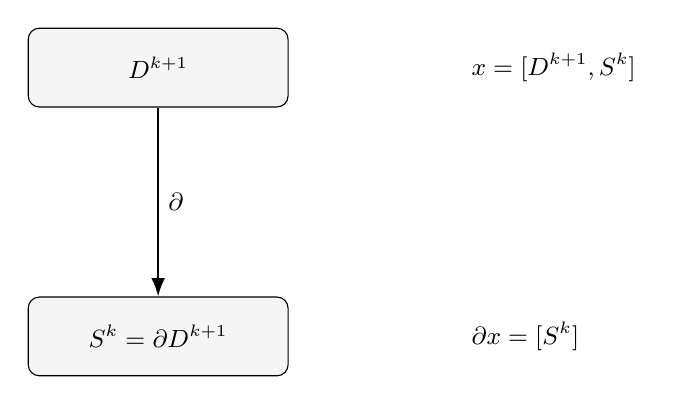
\begin{tikzpicture}[>=Latex, node distance=2.4cm, font=\small]
		\node[draw, rounded corners, minimum width=3.3cm, minimum height=1cm, fill=gray!8] (disk)
		{\(D^{k+1}\)};
		\node[draw, rounded corners, minimum width=3.3cm, minimum height=1cm, fill=gray!8, below=of disk] (sphere)
		{\(S^k=\partial D^{k+1}\)};
		\draw[->, thick] (disk) -- node[right] {\(\partial\)} (sphere);
		\node[right=2.2cm of disk] (x) {\(x=[D^{k+1},S^k]\)};
		\node[right=2.2cm of sphere] (bd) {\(\partial x=[S^k]\)};
	\end{tikzpicture}
\end{center}

This is the simplest topological version of Stokes' theorem:
\[
\int_{\partial c}\omega=\int_c d\omega.
\]

\subsection{Example 2. A filled triangle and its boundary circle}

Let
\[
X=\Delta^2,
\qquad
A=\partial\Delta^2.
\]
Topologically,
\[
\Delta^2\cong D^2,
\qquad
\partial\Delta^2\cong S^1.
\]
Let
\[
x=[\Delta^2,\partial\Delta^2]\in H_2(\Delta^2,\partial\Delta^2)
\]
be the relative fundamental class of the filled triangle. Its boundary is
\[
\partial x=[\partial\Delta^2]\in H_1(\partial\Delta^2).
\]

Choose
\[
a\in H^1(\partial\Delta^2)\cong \mathbb Z
\]
so that \(a\) evaluates to \(1\) on the positively oriented boundary loop:
\[
\langle a,[\partial\Delta^2]\rangle=1.
\]
Then
\[
\langle a,\partial x\rangle=1.
\]

The cohomology connecting map is
\[
\delta:H^1(\partial\Delta^2)
\longrightarrow
H^2(\Delta^2,\partial\Delta^2).
\]
Since
\[
H^2(\Delta^2,\partial\Delta^2)\cong\mathbb Z,
\]
the class \(\delta a\) is the relative generator. Therefore
\[
\langle \delta a,x\rangle=1.
\]

Hence
\[
\boxed{
	\langle a,\partial x\rangle=\langle \delta a,x\rangle.
}
\]

\begin{center}
	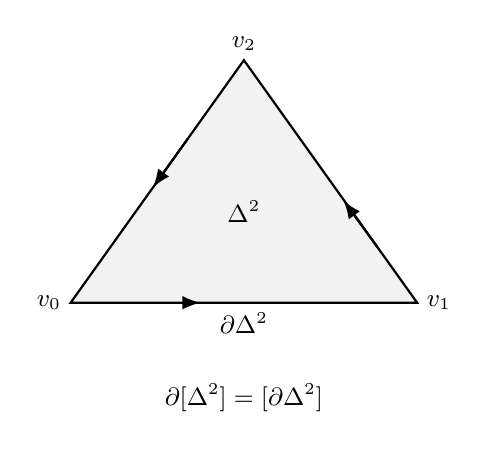
\begin{tikzpicture}[scale=1.1, >=Latex, font=\small]
		\coordinate (A) at (0,0);
		\coordinate (B) at (4,0);
		\coordinate (C) at (2,2.8);
		
		\fill[gray!10] (A)--(B)--(C)--cycle;
		\draw[thick] (A)--(B)--(C)--cycle;
		
		\draw[->, thick] (0.8,0) -- (1.5,0);
		\draw[->, thick] (3.55,0.63) -- (3.15,1.18);
		\draw[->, thick] (1.35,1.89) -- (0.95,1.33);
		
		\node at (2,1.05) {\(\Delta^2\)};
		\node[below] at (2,0) {\(\partial\Delta^2\)};
		\node[left] at (A) {\(v_0\)};
		\node[right] at (B) {\(v_1\)};
		\node[above] at (C) {\(v_2\)};
		
		\node[align=center] at (2,-1.1)
		{\(\partial[\Delta^2]=[\partial\Delta^2]\)};
	\end{tikzpicture}
\end{center}

The theorem says that evaluating a \(1\)-cohomology class on the boundary loop is the same as evaluating its connecting class on the filled triangle.

\subsection{Example 3. The annulus and the difference of two boundary circles}

Let
\[
X=S^1\times[0,1]
\]
be an annulus, and let
\[
A=\partial X
=
S^1\times\{0\}
\sqcup
S^1\times\{1\}.
\]
Thus \(A\) has two connected components: the inner boundary circle and the outer boundary circle.

The relative group is
\[
H_2(X,A)\cong\mathbb Z.
\]
Let
\[
x=[X,A]
\]
be the relative fundamental class of the annulus.

The boundary of the annulus is the difference of its two boundary circles:
\[
\partial x
=
[S^1\times\{1\}]
-
[S^1\times\{0\}].
\]
The minus sign appears because the two boundary components receive opposite induced orientations.

Now
\[
H^1(A)
\cong
H^1(S^1\sqcup S^1)
\cong
\mathbb Z\oplus\mathbb Z.
\]
A class
\[
a\in H^1(A)
\]
may therefore be written as
\[
a=(m,n),
\]
where \(m\) is the value on the outer boundary circle and \(n\) is the value on the inner boundary circle.

Then
\[
\langle a,\partial x\rangle
=
\left\langle
(m,n),
[S^1\times\{1\}]
-
[S^1\times\{0\}]
\right\rangle.
\]
Therefore
\[
\langle a,\partial x\rangle=m-n.
\]

Now consider the connecting homomorphism
\[
\delta:H^1(A)\longrightarrow H^2(X,A).
\]
Since
\[
H^2(X,A)\cong\mathbb Z,
\]
the class \(\delta a\) is determined by its value on the relative fundamental class \([X,A]\). By the compatibility identity from Problem 9,
\[
\langle \delta a,[X,A]\rangle
=
\langle a,\partial[X,A]\rangle
=
m-n.
\]
Hence
\[
\boxed{
	\langle \delta(m,n),[X,A]\rangle=m-n.
}
\]

Thus the connecting homomorphism detects the difference between the two boundary values:
\[
\boxed{
	\delta(m,n)=m-n.
}
\]

\begin{center}
	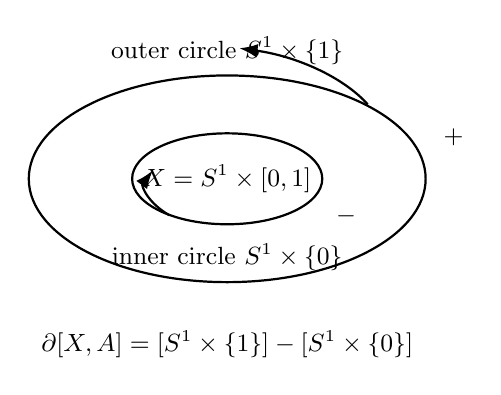
\begin{tikzpicture}[scale=1.05, >=Latex, font=\small]
		\draw[thick] (0,0) ellipse (2.4 and 1.25);
		\draw[thick] (0,0) ellipse (1.15 and 0.55);
		
		\node at (0,0) {\(X=S^1\times[0,1]\)};
		\node at (0,1.55) {outer circle \(S^1\times\{1\}\)};
		\node at (0,-0.95) {inner circle \(S^1\times\{0\}\)};
		
		\draw[->, thick] (1.7,0.9) arc[start angle=25,end angle=75,x radius=2.4,y radius=1.25];
		\draw[->, thick] (-0.7,-0.44) arc[start angle=220,end angle=160,x radius=1.15,y radius=0.55];
		
		\node[right] at (2.5,0.5) {\(+\)};
		\node[right] at (1.2,-0.45) {\(-\)};
		\node[align=center] at (0,-2.0)
		{\(\partial[X,A]=[S^1\times\{1\}]-[S^1\times\{0\}]\)};
	\end{tikzpicture}
\end{center}

This example is one of the clearest examples of a connecting homomorphism. The annulus has two boundary components. A cohomology class on the boundary gives two integers. The connecting map measures whether these two values agree.

\subsection{Example 4. The annulus as an obstruction example}

The annulus has
\[
H^1(X)\cong\mathbb Z.
\]
The boundary has
\[
H^1(A)\cong\mathbb Z\oplus\mathbb Z.
\]

The restriction map
\[
H^1(X)\longrightarrow H^1(A)
\]
sends a class
\[
r\in\mathbb Z
\]
to
\[
(r,r)\in\mathbb Z\oplus\mathbb Z.
\]
This means that a class on the annulus restricts to the same value on both boundary components.

Thus the image of the restriction map is the diagonal subgroup
\[
\{(r,r):r\in\mathbb Z\}\subseteq\mathbb Z\oplus\mathbb Z.
\]

The connecting homomorphism
\[
\delta:H^1(A)\longrightarrow H^2(X,A)
\]
kills exactly those pairs \((m,n)\) with \(m=n\). Therefore it measures the difference:
\[
\delta(m,n)=m-n.
\]

The relevant part of the long exact cohomology sequence becomes
\[
H^1(X)
\longrightarrow
H^1(A)
\xrightarrow{\delta}
H^2(X,A),
\]
or concretely,
\[
\mathbb Z
\longrightarrow
\mathbb Z\oplus\mathbb Z
\xrightarrow{m-n}
\mathbb Z.
\]

More explicitly,
\[
r\longmapsto (r,r),
\]
and
\[
(m,n)\longmapsto m-n.
\]
Since
\[
m-n=0
\quad\Longleftrightarrow\quad
m=n,
\]
we have
\[
\ker(\delta)=\operatorname{im}\bigl(H^1(X)\to H^1(A)\bigr).
\]
This is exactly the meaning of exactness.

\begin{center}
	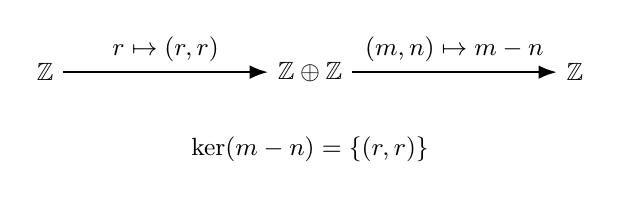
\begin{tikzpicture}[>=Latex, node distance=2.6cm, font=\small]
		\node (Z1) {\(\mathbb Z\)};
		\node[right=of Z1] (Z2) {\(\mathbb Z\oplus\mathbb Z\)};
		\node[right=of Z2] (Z3) {\(\mathbb Z\)};
		\draw[->, thick] (Z1) -- node[above] {\(r\mapsto(r,r)\)} (Z2);
		\draw[->, thick] (Z2) -- node[above] {\((m,n)\mapsto m-n\)} (Z3);
		\node[below=0.45cm of Z2] {\(\ker(m-n)=\{(r,r)\}\)};
	\end{tikzpicture}
\end{center}

So this example illustrates the slogan:
\[
\boxed{
	\delta \text{ measures the obstruction to extending boundary data into the interior.}
}
\]

\subsection{Example 5. The Bockstein for \texorpdfstring{\(S^1\)}{S1}: a zero example}

Consider the coefficient sequence
\[
0\longrightarrow \mathbb Z
\xrightarrow{\times 2}
\mathbb Z
\longrightarrow
\mathbb Z/2
\longrightarrow 0.
\]
The associated Bockstein is
\[
\beta:H_q(S^1;\mathbb Z/2)
\longrightarrow
H_{q-1}(S^1;\mathbb Z).
\]

The cellular chain complex of \(S^1\) with integral coefficients is
\[
0
\longrightarrow
C_1(S^1;\mathbb Z)
\xrightarrow{0}
C_0(S^1;\mathbb Z)
\longrightarrow
0.
\]
Since \(S^1\) has one \(0\)-cell and one \(1\)-cell, this is
\[
0
\longrightarrow
\mathbb Z
\xrightarrow{0}
\mathbb Z
\longrightarrow
0.
\]

With \(\mathbb Z/2\)-coefficients, the chain complex is
\[
0
\longrightarrow
\mathbb Z/2
\xrightarrow{0}
\mathbb Z/2
\longrightarrow
0.
\]

Let
\[
[e^1]\in H_1(S^1;\mathbb Z/2)
\]
be the generator represented by the mod \(2\) \(1\)-cell. Lift it to the integral \(1\)-cell
\[
e^1\in C_1(S^1;\mathbb Z).
\]
Its boundary is
\[
\partial e^1=0.
\]
Therefore
\[
\beta([e^1])=0.
\]

Thus
\[
\boxed{
	\beta:H_1(S^1;\mathbb Z/2)\longrightarrow H_0(S^1;\mathbb Z)
	\text{ is zero.}
}
\]

This makes sense because the mod \(2\) fundamental class of \(S^1\) comes directly from an integral fundamental class. There is no hidden \(2\)-torsion for the Bockstein to detect.

\subsection{Example 6. The Bockstein for \texorpdfstring{\(\mathbb{RP}^2\)}{RP2}: a nonzero example}

This is the most important basic Bockstein example.

The real projective plane has a CW structure with one cell in each dimension \(0,1,2\):
\[
\mathbb{RP}^2=e^0\cup e^1\cup e^2.
\]
The cellular chain complex with integer coefficients is
\[
0
\longrightarrow
C_2
\xrightarrow{d_2}
C_1
\xrightarrow{d_1}
C_0
\longrightarrow
0,
\]
where
\[
C_2\cong C_1\cong C_0\cong\mathbb Z,
\]
and
\[
d_2=\times 2,
\qquad
d_1=0.
\]
Thus the complex is
\[
0
\longrightarrow
\mathbb Z
\xrightarrow{\times 2}
\mathbb Z
\xrightarrow{0}
\mathbb Z
\longrightarrow
0.
\]

Therefore
\[
H_2(\mathbb{RP}^2;\mathbb Z)=0,
\]
\[
H_1(\mathbb{RP}^2;\mathbb Z)\cong\mathbb Z/2,
\]
and
\[
H_0(\mathbb{RP}^2;\mathbb Z)\cong\mathbb Z.
\]

With \(\mathbb Z/2\)-coefficients, multiplication by \(2\) becomes zero, so the mod \(2\) cellular chain complex is
\[
0
\longrightarrow
\mathbb Z/2
\xrightarrow{0}
\mathbb Z/2
\xrightarrow{0}
\mathbb Z/2
\longrightarrow
0.
\]
Hence
\[
H_2(\mathbb{RP}^2;\mathbb Z/2)\cong\mathbb Z/2,
\]
\[
H_1(\mathbb{RP}^2;\mathbb Z/2)\cong\mathbb Z/2,
\]
and
\[
H_0(\mathbb{RP}^2;\mathbb Z/2)\cong\mathbb Z/2.
\]

Now compute the Bockstein
\[
\beta:H_2(\mathbb{RP}^2;\mathbb Z/2)
\longrightarrow
H_1(\mathbb{RP}^2;\mathbb Z).
\]

Let
\[
[e^2]\in H_2(\mathbb{RP}^2;\mathbb Z/2)
\]
be the mod \(2\) class represented by the \(2\)-cell. Lift \(e^2\) to the integral chain
\[
e^2\in C_2(\mathbb{RP}^2;\mathbb Z).
\]
Its integral boundary is
\[
\partial e^2=2e^1.
\]
Since this boundary is divisible by \(2\), we divide by \(2\):
\[
\frac{1}{2}\partial e^2=e^1.
\]
Therefore
\[
\beta([e^2])=[e^1].
\]
But \([e^1]\) generates
\[
H_1(\mathbb{RP}^2;\mathbb Z)\cong\mathbb Z/2.
\]
Thus
\[
\boxed{
	\beta:H_2(\mathbb{RP}^2;\mathbb Z/2)
	\longrightarrow
	H_1(\mathbb{RP}^2;\mathbb Z)
}
\]
is an isomorphism.

\begin{center}
	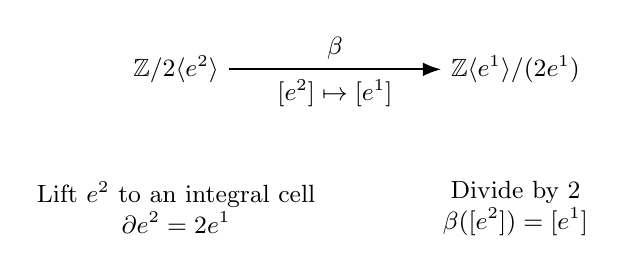
\begin{tikzpicture}[>=Latex, node distance=2.7cm, font=\small]
		\node (C2) {\(\mathbb Z/2\langle e^2\rangle\)};
		\node[right=of C2] (C1) {\(\mathbb Z\langle e^1\rangle/(2e^1)\)};
		\draw[->, thick] (C2) -- node[above] {\(\beta\)} node[below] {\([e^2]\mapsto[e^1]\)} (C1);
		
		\node[below=1cm of C2, align=center] (lift)
		{Lift \(e^2\) to an integral cell\\ \(\partial e^2=2e^1\)};
		\node[below=1cm of C1, align=center] (divide)
		{Divide by \(2\)\\ \(\beta([e^2])=[e^1]\)};
	\end{tikzpicture}
\end{center}

This example explains why the top mod \(2\) class of \(\mathbb{RP}^2\) is important even though
\[
H_2(\mathbb{RP}^2;\mathbb Z)=0.
\]
The top mod \(2\) class detects the integral torsion class in degree \(1\):
\[
H_2(\mathbb{RP}^2;\mathbb Z/2)
\xrightarrow{\beta}
H_1(\mathbb{RP}^2;\mathbb Z).
\]

\subsection{Example 7. The Bockstein for \texorpdfstring{\(\mathbb{RP}^3\)}{RP3}}

Now consider
\[
\mathbb{RP}^3.
\]
It has one cell in each dimension \(0,1,2,3\). Its cellular chain complex with integral coefficients is
\[
0
\longrightarrow
C_3
\xrightarrow{d_3}
C_2
\xrightarrow{d_2}
C_1
\xrightarrow{d_1}
C_0
\longrightarrow
0,
\]
where each \(C_i\cong\mathbb Z\), and
\[
d_3=0,
\qquad
d_2=\times 2,
\qquad
d_1=0.
\]
Thus
\[
0
\longrightarrow
\mathbb Z
\xrightarrow{0}
\mathbb Z
\xrightarrow{\times 2}
\mathbb Z
\xrightarrow{0}
\mathbb Z
\longrightarrow
0.
\]

Hence
\[
H_3(\mathbb{RP}^3;\mathbb Z)\cong\mathbb Z,
\]
\[
H_2(\mathbb{RP}^3;\mathbb Z)=0,
\]
\[
H_1(\mathbb{RP}^3;\mathbb Z)\cong\mathbb Z/2,
\]
and
\[
H_0(\mathbb{RP}^3;\mathbb Z)\cong\mathbb Z.
\]

With \(\mathbb Z/2\)-coefficients, all cellular boundary maps vanish, so
\[
H_q(\mathbb{RP}^3;\mathbb Z/2)\cong\mathbb Z/2
\qquad
\text{for }q=0,1,2,3.
\]

Now consider the Bockstein
\[
\beta:H_2(\mathbb{RP}^3;\mathbb Z/2)
\longrightarrow
H_1(\mathbb{RP}^3;\mathbb Z).
\]
The mod \(2\) class \([e^2]\) lifts to the integral \(2\)-cell \(e^2\), and
\[
\partial e^2=2e^1.
\]
Therefore
\[
\beta([e^2])=[e^1].
\]
Thus
\[
\boxed{
	\beta:H_2(\mathbb{RP}^3;\mathbb Z/2)
	\longrightarrow
	H_1(\mathbb{RP}^3;\mathbb Z)
}
\]
is an isomorphism.

But now the top class behaves differently. Consider
\[
\beta:H_3(\mathbb{RP}^3;\mathbb Z/2)
\longrightarrow
H_2(\mathbb{RP}^3;\mathbb Z).
\]
Since
\[
H_2(\mathbb{RP}^3;\mathbb Z)=0,
\]
this Bockstein is zero.

Moreover, the top mod \(2\) class comes from reducing the integral fundamental class:
\[
H_3(\mathbb{RP}^3;\mathbb Z)\cong\mathbb Z
\longrightarrow
H_3(\mathbb{RP}^3;\mathbb Z/2)\cong\mathbb Z/2.
\]

Thus \(\mathbb{RP}^3\) shows both phenomena:
\[
\boxed{
	H_2(-;\mathbb Z/2)\text{ detects torsion below via Bockstein,}
}
\]
but
\[
\boxed{
	H_3(-;\mathbb Z/2)\text{ comes from the integral fundamental class.}
}
\]

\subsection{Example 8. Naturality of the Bockstein for maps of \texorpdfstring{\(\mathbb{RP}^2\)}{RP2}}

Let
\[
f:\mathbb{RP}^2\longrightarrow \mathbb{RP}^2
\]
be a continuous map. Naturality of the Bockstein says that the diagram
\[
\begin{array}{ccc}
	H_2(\mathbb{RP}^2;\mathbb Z/2)
	&
	\xrightarrow{\beta}
	&
	H_1(\mathbb{RP}^2;\mathbb Z)
	\\[1mm]
	\downarrow f_*
	&&
	\downarrow f_*
	\\[1mm]
	H_2(\mathbb{RP}^2;\mathbb Z/2)
	&
	\xrightarrow{\beta}
	&
	H_1(\mathbb{RP}^2;\mathbb Z)
\end{array}
\]
commutes. Equivalently,
\[
f_*\beta=\beta f_*.
\]

Let
\[
u\in H_2(\mathbb{RP}^2;\mathbb Z/2)
\]
be the generator, and let
\[
v\in H_1(\mathbb{RP}^2;\mathbb Z)
\]
be the generator. We know from the previous example that
\[
\beta(u)=v.
\]

If \(f\) is the identity map, then both vertical maps are the identity, and
\[
f_*\beta(u)=f_*(v)=v,
\]
while
\[
\beta f_*(u)=\beta(u)=v.
\]
Thus
\[
f_*\beta(u)=\beta f_*(u).
\]

Now take a constant map
\[
c:\mathbb{RP}^2\longrightarrow \mathbb{RP}^2.
\]
A constant map kills positive-dimensional homology. Therefore
\[
c_*u=0
\]
and
\[
c_*v=0.
\]
Then
\[
c_*\beta(u)=c_*(v)=0,
\]
while
\[
\beta c_*(u)=\beta(0)=0.
\]
So again
\[
c_*\beta(u)=\beta c_*(u).
\]

This shows concretely that \(f\) cannot move the mod \(2\) class \(u\) and the integral torsion class \(v\) independently. The Bockstein forces them to be compatible.

\subsection{Example 9. Even-dimensional projective space: \texorpdfstring{\(\mathbb{RP}^2\)}{RP2}}

This example explains why the converse statement in Problem 10 holds when \(n\) is even.

For \(\mathbb{RP}^2\), the integral homology groups are
\[
H_0(\mathbb{RP}^2;\mathbb Z)\cong\mathbb Z,
\]
\[
H_1(\mathbb{RP}^2;\mathbb Z)\cong\mathbb Z/2,
\]
and
\[
H_2(\mathbb{RP}^2;\mathbb Z)=0.
\]

The mod \(2\) homology groups are
\[
H_0(\mathbb{RP}^2;\mathbb Z/2)\cong\mathbb Z/2,
\]
\[
H_1(\mathbb{RP}^2;\mathbb Z/2)\cong\mathbb Z/2,
\]
and
\[
H_2(\mathbb{RP}^2;\mathbb Z/2)\cong\mathbb Z/2.
\]

Suppose we know
\[
f_*:H_*(\mathbb{RP}^2;\mathbb Z/2)
\longrightarrow
H_*(\mathbb{RP}^2;\mathbb Z/2).
\]
Can we recover the integral homology action?

Yes.

In degree \(0\), the answer is automatic because \(\mathbb{RP}^2\) is connected:
\[
f_*=\operatorname{id}
\qquad
\text{on }
H_0(\mathbb{RP}^2;\mathbb Z).
\]

In degree \(1\), the reduction map
\[
H_1(\mathbb{RP}^2;\mathbb Z)
\longrightarrow
H_1(\mathbb{RP}^2;\mathbb Z/2)
\]
is an isomorphism:
\[
\mathbb Z/2\cong \mathbb Z/2.
\]
Therefore the mod \(2\) action determines the integral action in degree \(1\).

In degree \(2\), there is no integral homology group:
\[
H_2(\mathbb{RP}^2;\mathbb Z)=0.
\]
So there is nothing extra to recover.

Therefore the mod \(2\) homology action determines the integral homology action for \(\mathbb{RP}^2\).

This is the general even-dimensional situation:
\[
\boxed{
	\mathbb{RP}^{2m}
	\text{ has no top } \mathbb Z\text{-homology, so mod }2\text{ sees all the integral homology action.}
}
\]

\subsection{Example 10. Odd-dimensional projective space: \texorpdfstring{\(\mathbb{RP}^3\)}{RP3}}

Now take
\[
\mathbb{RP}^3.
\]
Its integral homology is
\[
H_0(\mathbb{RP}^3;\mathbb Z)\cong\mathbb Z,
\]
\[
H_1(\mathbb{RP}^3;\mathbb Z)\cong\mathbb Z/2,
\]
\[
H_2(\mathbb{RP}^3;\mathbb Z)=0,
\]
and
\[
H_3(\mathbb{RP}^3;\mathbb Z)\cong\mathbb Z.
\]

Its mod \(2\) homology is
\[
H_q(\mathbb{RP}^3;\mathbb Z/2)\cong\mathbb Z/2
\qquad
\text{for }q=0,1,2,3.
\]

Compare two maps:
\[
\operatorname{id}:\mathbb{RP}^3\longrightarrow\mathbb{RP}^3
\]
and an orientation-reversing projective linear homeomorphism
\[
r:\mathbb{RP}^3\longrightarrow\mathbb{RP}^3.
\]

On top integral homology,
\[
H_3(\mathbb{RP}^3;\mathbb Z)\cong\mathbb Z,
\]
the identity acts by
\[
(\operatorname{id})_*=+1,
\]
whereas the orientation-reversing homeomorphism acts by
\[
r_*=-1.
\]
Thus the two maps are different on integral homology.

However, over \(\mathbb Z/2\),
\[
+1=-1.
\]
Therefore on top mod \(2\) homology,
\[
H_3(\mathbb{RP}^3;\mathbb Z/2)\cong\mathbb Z/2,
\]
both maps act in the same way.

Also, on
\[
H_1(\mathbb{RP}^3;\mathbb Z/2)\cong\mathbb Z/2,
\]
any isomorphism must be the identity, because \(\mathbb Z/2\) has only one nonzero element.

Hence the identity map and an orientation-reversing homeomorphism have the same action on mod \(2\) homology but different actions on integral homology.

Therefore
\[
\boxed{
	\text{for odd }n,\text{ mod }2\text{ homology cannot distinguish }+1\text{ from }-1
}
\]
on the top integral homology group
\[
H_n(\mathbb{RP}^n;\mathbb Z)\cong\mathbb Z.
\]

This is exactly why the converse fails when \(n\) is odd.

\subsection{Example 11. Summary table of the main examples}

\begin{center}
	\renewcommand{\arraystretch}{1.35}
	\begin{tabular}{|>{\centering\arraybackslash}p{0.08\textwidth}|
			>{\centering\arraybackslash}p{0.24\textwidth}|
			>{\centering\arraybackslash}p{0.31\textwidth}|
			>{\arraybackslash}p{0.27\textwidth}|}
		\hline
		\textbf{Example}
		&
		\textbf{Space or pair}
		&
		\textbf{Important map}
		&
		\textbf{Meaning}
		\\
		\hline
		1
		&
		\((D^{k+1},S^k)\)
		&
		\(\delta:H^k(S^k)\to H^{k+1}(D^{k+1},S^k)\)
		&
		The boundary sphere corresponds to the relative coboundary.
		\\
		\hline
		2
		&
		\((\Delta^2,\partial\Delta^2)\)
		&
		\(\langle a,\partial x\rangle=\langle\delta a,x\rangle\)
		&
		The filled triangle gives the simplest finite-dimensional Stokes-type example.
		\\
		\hline
		3
		&
		\((S^1\times[0,1],\partial)\)
		&
		\(\delta(m,n)=m-n\)
		&
		The annulus detects the difference of two boundary values.
		\\
		\hline
		4
		&
		\(S^1\)
		&
		\(\beta=0\)
		&
		The mod \(2\) class lifts to an integral class, so no torsion is detected.
		\\
		\hline
		5
		&
		\(\mathbb{RP}^2\)
		&
		\(\beta:H_2(-;\mathbb Z/2)\to H_1(-;\mathbb Z)\)
		&
		The top mod \(2\) class detects the \(\mathbb Z/2\)-torsion class below.
		\\
		\hline
		6
		&
		\(\mathbb{RP}^3\)
		&
		\(\beta:H_2(-;\mathbb Z/2)\to H_1(-;\mathbb Z)\)
		&
		The Bockstein detects lower torsion, while the top class comes from integral homology.
		\\
		\hline
		7
		&
		\(\mathbb{RP}^{2m}\)
		&
		\(H_*(-;\mathbb Z/2)\Rightarrow H_*(-;\mathbb Z)\)
		&
		The converse holds because there is no top integral \(\mathbb Z\)-class.
		\\
		\hline
		8
		&
		\(\mathbb{RP}^{2m+1}\)
		&
		\(+1\) versus \(-1\) on top \(H_n\)
		&
		The converse fails because mod \(2\) cannot distinguish signs.
		\\
		\hline
	\end{tabular}
\end{center}

\subsection{Final intuition}

Problem 9 is about the principle
\[
\boxed{
	\text{boundary on chains corresponds to coboundary on cochains.}
}
\]
In formula form:
\[
\boxed{
	\langle a,\partial x\rangle=\langle \delta a,x\rangle.
}
\]
This is the algebraic-topological version of Stokes' theorem:
\[
\int_{\partial c}\omega=\int_c d\omega.
\]

Problem 10 is about the principle
\[
\boxed{
	\text{changing coefficients creates connecting maps that detect hidden torsion.}
}
\]
The most important coefficient sequence is
\[
0\longrightarrow \mathbb Z
\xrightarrow{\times 2}
\mathbb Z
\longrightarrow
\mathbb Z/2
\longrightarrow 0.
\]
Its Bockstein homomorphism
\[
\beta:H_q(X;\mathbb Z/2)
\longrightarrow
H_{q-1}(X;\mathbb Z)
\]
takes a mod \(2\) class, lifts it to an integral chain, computes its integral boundary, and records the divided boundary.

The best geometric example for Problem 9 is
\[
(D^{k+1},S^k),
\]
because the boundary of the disk is literally the sphere.

The best algebraic-topological example for Problem 10 is
\[
\mathbb{RP}^2,
\]
because the mod \(2\) top class detects the integral torsion class through the Bockstein:
\[
\boxed{
	\beta([e^2])=[e^1].
}
\]

Thus the two problems together show how long exact sequences connect geometry, algebra, and evaluation pairings.


\section{Visual diagrams for Problems 9--10}

This section collects diagrams and charts illustrating the two key mechanisms used in Problems 9--10:
\[
\langle a,\partial x\rangle=\langle \delta a,x\rangle
\]
and
\[
f_*\beta_X=\beta_Yf_*.
\]
The figures are intended to be inserted after the theory section or after the examples section.

\subsection{Pairing and boundary for \texorpdfstring{$(D^{k+1},S^k)$}{(D^{k+1}, S^k)}}

The pair
\[
(D^{k+1},S^k)=(D^{k+1},\partial D^{k+1})
\]
is the cleanest geometric model for the compatibility identity
\[
\langle a,\partial x\rangle=\langle \delta a,x\rangle .
\]
The relative class
\[
x=[D^{k+1},S^k]\in H_{k+1}(D^{k+1},S^k)
\]
has boundary
\[
\partial x=[S^k]\in H_k(S^k).
\]
Therefore evaluating a class on the boundary sphere is the same as evaluating the connecting cohomology class on the relative disk class.

\begin{figure}[H]
	\centering
	
\includegraphics[width=0.96\textwidth]{figures/Downloads_figures_fig_pairing_boundary_disk_sphere.png}
	\caption{The relative Stokes principle for the pair \((D^{k+1},S^k)\). The identity \(\langle a,\partial x\rangle=\langle \delta a,x\rangle\) says that the homology boundary and the cohomology connecting map are adjoint under the Kronecker pairing.}
	\label{fig:pairing-boundary-disk-sphere}
\end{figure}

\subsection{Annulus example and the obstruction map \texorpdfstring{$\delta(m,n)=m-n$}{delta(m,n)=m-n}}

Let
\[
X=S^1\times[0,1],
\qquad
A=\partial X=S^1\times\{0\}\sqcup S^1\times\{1\}.
\]
The boundary of the relative fundamental class is
\[
\partial[X,A]=[S^1\times\{1\}]-[S^1\times\{0\}].
\]
Since
\[
H^1(A)\cong H^1(S^1\sqcup S^1)\cong \mathbb Z\oplus\mathbb Z,
\]
a class on the boundary may be written as a pair
\[
(m,n),
\]
where the two entries record the values on the two boundary components. The connecting homomorphism measures the failure of these values to agree:
\[
\delta(m,n)=m-n.
\]
Thus the annulus gives a very concrete obstruction interpretation of the connecting homomorphism.

\begin{figure}[H]
	\centering
	
\includegraphics[width=0.96\textwidth]{figures/Downloads_figures_fig_annulus_connecting_map.png}
	\caption{The annulus example. A cohomology class on the boundary has two integer values, one on each boundary component. The connecting map detects their difference: \(\delta(m,n)=m-n\).}
	\label{fig:annulus-connecting-map}
\end{figure}

\subsection{The Bockstein homomorphism for \texorpdfstring{$\mathbb{RP}^2$}{RP2}}

For the coefficient sequence
\[
0\longrightarrow \mathbb Z
\xrightarrow{\times 2}
\mathbb Z
\longrightarrow
\mathbb Z/2
\longrightarrow 0,
\]
the Bockstein homomorphism is
\[
\beta:H_q(X;\mathbb Z/2)\longrightarrow H_{q-1}(X;\mathbb Z).
\]
For \(X=\mathbb{RP}^2\), the cellular chain complex over \(\mathbb Z\) contains the boundary map
\[
C_2(\mathbb{RP}^2;\mathbb Z)
\xrightarrow{\times 2}
C_1(\mathbb{RP}^2;\mathbb Z).
\]
Therefore, if \([e^2]\) denotes the mod \(2\) top cell class, then lifting it to an integral \(2\)-cell gives
\[
\partial e^2=2e^1.
\]
The Bockstein divides this boundary by \(2\), giving
\[
\beta([e^2])=[e^1].
\]
Hence
\[
\beta:H_2(\mathbb{RP}^2;\mathbb Z/2)	o H_1(\mathbb{RP}^2;\mathbb Z)
\]
is an isomorphism.

\begin{figure}[H]
	\centering
	
\includegraphics[width=0.96\textwidth]{figures/Downloads_figures_fig_bockstein_rp2.png}
	\caption{The Bockstein homomorphism for \(\mathbb{RP}^2\). The mod \(2\) top cell detects the integral \(\mathbb Z/2\)-torsion class one dimension lower.}
	\label{fig:bockstein-rp2}
\end{figure}

\subsection{Even versus odd real projective spaces}

The parity of \(n\) matters because
\[
\mathbb{RP}^n \text{ is orientable if and only if } n \text{ is odd}.
\]
For even-dimensional projective space,
\[
H_{2m}(\mathbb{RP}^{2m};\mathbb Z)=0,
\]
so there is no top-dimensional integral \(\mathbb Z\)-class. Consequently, the mod \(2\) action determines the integral action.

For odd-dimensional projective space,
\[
H_{2m+1}(\mathbb{RP}^{2m+1};\mathbb Z)\cong\mathbb Z.
\]
On this top homology group, two maps may differ by multiplication by \(+1\) or \(-1\). But after reducing modulo \(2\), these two signs become equal:
\[
+1\equiv -1\pmod 2.
\]
Therefore the converse fails in odd dimensions: the mod \(2\) homology action does not determine the full integral action.

\begin{figure}[H]
	\centering
	
\includegraphics[width=0.96\textwidth]{figures/Downloads_figures_fig_even_vs_odd_rpn.png}
	\caption{Comparison of even and odd real projective spaces. In even dimensions there is no top integral \(\mathbb Z\)-class, so the mod \(2\) action determines the integral action. In odd dimensions, the top integral class is \(\mathbb Z\), and mod \(2\) cannot distinguish \(+1\) from \(-1\).}
	\label{fig:even-vs-odd-projective-spaces}
\end{figure}

\subsection{How to reference the figures in the text}

You can refer to the disk--sphere model using Figure~\ref{fig:pairing-boundary-disk-sphere}. The annulus obstruction example is Figure~\ref{fig:annulus-connecting-map}. The Bockstein computation for \(\mathbb{RP}^2\) is Figure~\ref{fig:bockstein-rp2}. The parity comparison for \(\mathbb{RP}^n\) is Figure~\ref{fig:even-vs-odd-projective-spaces}.


\end{document}


